%%%%%%%%%%%%%%%%%%%%%%%%%%%%%%%%%%%%%%%%%
% Masters/Doctoral Thesis 
% LaTeX Template
% Version 2.5 (27/8/17)
%
% This template was downloaded from:
% http://www.LaTeXTemplates.com
%
% Version 2.x major modifications by:
% Vel (vel@latextemplates.com)
%
% This template is based on a template by:
% Steve Gunn (http://users.ecs.soton.ac.uk/srg/softwaretools/document/templates/)
% Sunil Patel (http://www.sunilpatel.co.uk/thesis-template/)
%
% Template license:
% CC BY-NC-SA 3.0 (http://creativecommons.org/licenses/by-nc-sa/3.0/)
%
%%%%%%%%%%%%%%%%%%%%%%%%%%%%%%%%%%%%%%%%%

%----------------------------------------------------------------------------------------
%	PACKAGES AND OTHER DOCUMENT CONFIGURATIONS
%----------------------------------------------------------------------------------------

\documentclass[
11pt, % The default document font size, options: 10pt, 11pt, 12pt
%oneside, % Two side (alternating margins) for binding by default, uncomment to switch to one side
english, % ngerman for German
onehalfspacing %onehalfspacing %singlespacing, % Single line spacing, alternatives: onehalfspacing or doublespacing
%draft, % Uncomment to enable draft mode (no pictures, no links, overfull hboxes indicated)
%nolistspacing, % If the document is onehalfspacing or doublespacing, uncomment this to set spacing in lists to single
%liststotoc, % Uncomment to add the list of figures/tables/etc to the table of contents
%toctotoc, % Uncomment to add the main table of contents to the table of contents
parskip, % Uncomment to add space between paragraphs
%nohyperref, % Uncomment to not load the hyperref package
headsepline, % Uncomment to get a line under the header
%chapterinoneline, % Uncomment to place the chapter title next to the number on one line
%consistentlayout, % Uncomment to change the layout of the declaration, abstract and acknowledgements pages to match the default layout
]{MastersDoctoralThesis} % The class file specifying the document structure

\usepackage{amsmath}
\usepackage{algpseudocode}
\usepackage{algorithm}


\algnewcommand\algorithmicforeach{\textbf{for each}}
\algdef{S}[FOR]{ForEach}[1]{\algorithmicforeach\ #1\ \algorithmicdo}

\makeatletter
\def\BState{\State\hskip-\ALG@thistlm}
\makeatother

\setlength{\parskip}{1.5em}


\usepackage[utf8]{inputenc} % Required for inputting international characters
\usepackage[T1]{fontenc} % Output font encoding for international characters

\usepackage{mathpazo} % Use the Palatino font by default
\usepackage{siunitx}
\usepackage[backend=bibtex,style=authoryear,natbib=true]{biblatex} % Use the bibtex backend with the authoryear citation style (which resembles APA)



\usepackage{titlesec}

\setcounter{secnumdepth}{5}

\titleformat{\paragraph}
{\normalfont\normalsize\bfseries}{\theparagraph}{1em}{}
\titlespacing*{\paragraph}
{0pt}{3.25ex plus 1ex minus .2ex}{1.5ex plus .2ex}

\titleformat{\subparagraph}
{\normalfont\normalsize\bfseries}{\thesubparagraph}{1em}{}
\titlespacing*{\subparagraph}
{0pt}{3.25ex plus 1ex minus .2ex}{1.5ex plus .2ex}

\addbibresource{example.bib} % The filename of the bibliography

\usepackage[autostyle=true]{csquotes} % Required to generate language-dependent quotes in the bibliography

%----------------------------------------------------------------------------------------
%	MARGIN SETTINGS
%----------------------------------------------------------------------------------------

\geometry{
	paper=a4paper, % Change to letterpaper for US letter
	inner=2.5cm, % Inner margin
	outer=3.8cm, % Outer margin
	bindingoffset=.5cm, % Binding offset
	top=1.5cm, % Top margin
	bottom=1.5cm, % Bottom margin
	%showframe, % Uncomment to show how the type block is set on the page
}

%----------------------------------------------------------------------------------------
%	THESIS INFORMATION
%----------------------------------------------------------------------------------------

\thesistitle{Interactive visualization for volumetric datasets } % Your thesis title, this is used in the title and abstract, print it elsewhere with \ttitle
\supervisor{Christophe \textsc{Hurter}} % Your supervisor's name, this is used in the title page, print it elsewhere with \supname
\examiner{} % Your examiner's name, this is not currently used anywhere in the template, print it elsewhere with \examname
\degree{Doctor of Philosophy} % Your degree name, this is used in the title page and abstract, print it elsewhere with \degreename
\author{Michael \textsc{Traor\'e}} % Your name, this is used in the title page and abstract, print it elsewhere with \authorname
\addresses{} % Your address, this is not currently used anywhere in the template, print it elsewhere with \addressname

\subject{Computer Science} % Your subject area, this is not currently used anywhere in the template, print it elsewhere with \subjectname
\keywords{} % Keywords for your thesis, this is not currently used anywhere in the template, print it elsewhere with \keywordnames
\university{\href{https://www.isae-supaero.fr/en/}{Institut supérieur de l'aéronautique et de l'espace (ISAE-SUPAERO)}} % Your university's name and URL, this is used in the title page and abstract, print it elsewhere with \univname
\department{\href{http://www.enac.fr}{\'Ecole Nationale de l'Aviation Civile (ENAC)}} % Your department's name and URL, this is used in the title page and abstract, print it elsewhere with \deptname
\group{\href{http://devi.recherche.enac.fr}{Data Economics and Interactive Visualization (DEVI)}} % Your research group's name and URL, this is used in the title page, print it elsewhere with \groupname
\faculty{\href{https://www.adum.fr/as/ed/page.pl?site=edsys&page=accueil}{\'Ecole Doctorale Syst\`emes (EDSYS)}} % Your faculty's name and URL, this is used in the title page and abstract, print it elsewhere with \facname

\AtBeginDocument{
\hypersetup{pdftitle=\ttitle} % Set the PDF's title to your title
\hypersetup{pdfauthor=\authorname} % Set the PDF's author to your name
\hypersetup{pdfkeywords=\keywordnames} % Set the PDF's keywords to your keywords
}


\usepackage{amssymb}
\usepackage{array,longtable}

\newcounter{mquestion}
\newcounter{row}

\makeatletter
\newtoks\@tabtoks
\newcommand\addtabtoks[1]{\@tabtoks\expandafter{\the\@tabtoks#1}}
\newcommand*\resettabtoks{\@tabtoks{}}
\newcommand*\printtabtoks{\the\@tabtoks}
\makeatother

\newcommand\CheckTable[1]{%
  \setcounter{mquestion}{0}
  \setcounter{row}{0}
  \resettabtoks
  \loop\ifnum\therow<#1\relax
    \stepcounter{row}
    \addtabtoks{& $\square$ & $\square$ & $\square$ & $\square$ & $\square$ \\}%
  \repeat
  \begin{longtable}{>{\stepcounter{mquestion}}l*{5}{c}}
    \multicolumn{1}{c}{} & Bad & Not Bad & Neutral & OK & Good \\
    \printtabtoks
  \end{longtable}%
}


\newcommand\CheckTablelevel[1]{%
  \setcounter{mquestion}{0}
  \setcounter{row}{0}
  \resettabtoks
  \loop\ifnum\therow<#1\relax
    \stepcounter{row}
    \addtabtoks{& $\square$ & $\square$ & $\square$ & $\square$ & $\square$ \\}%
  \repeat
  \begin{longtable}{>{\stepcounter{mquestion}}l*{5}{c}}
    \multicolumn{1}{c}{} & Novice &  Adv. Beginner &  Competent & Proficient  & Expert \\
    \printtabtoks
  \end{longtable}%
}

\newcommand\CheckTableDifficulty[1]{%
  \setcounter{mquestion}{0}
  \setcounter{row}{0}
  \resettabtoks
  \loop\ifnum\therow<#1\relax
    \stepcounter{row}
    \addtabtoks{& $\square$ & $\square$ & $\square$ & $\square$ & $\square$ \\}%
  \repeat
  \begin{longtable}{>{\stepcounter{mquestion}}l*{5}{c}}
    \multicolumn{1}{c}{} & Easy & Quite Easy & Neutral & Quite Hard & Hard \\
    \printtabtoks
  \end{longtable}%
}


\usepackage{xpatch}% http://ctan.org/pkg/etoolbox
\xpatchcmd{\answerline}% <cmd>
  {\par\nobreak\vskip\answerskip}% <search>
  {}% <replace>
  {}{}% <success><failure>

\newcommand{\leftanswerline}[1][]%
{\ifthenelse{\equal{#1}{}}%
{\par\hspace{-1.3em}\begin{minipage}{1em}\answerline\end{minipage}}%
{\par\hspace{-1.3em}\begin{minipage}{1em}\answerline[#1]\end{minipage}}%
}

\begin{document}

\frontmatter % Use roman page numbering style (i, ii, iii, iv...) for the pre-content pages

\pagestyle{plain} % Default to the plain heading style until the thesis style is called for the body content

%----------------------------------------------------------------------------------------
%	TITLE PAGE
%----------------------------------------------------------------------------------------

\begin{titlepage}
\begin{center}

\vspace*{.06\textheight}
{\scshape\LARGE \univname\par}\vspace{1.5cm} % University name
\textsc{\Large Doctoral Thesis}\\[0.5cm] % Thesis type

\HRule \\[0.4cm] % Horizontal line
{\huge \bfseries \ttitle\par}\vspace{0.4cm} % Thesis title
\HRule \\[1.5cm] % Horizontal line
 
\begin{minipage}[t]{0.4\textwidth}
\begin{flushleft} \large
\emph{Author:}\\
\href{https://www.linkedin.com/in/michael-traor%C3%A9-1a620596/}{\authorname} % Author name - remove the \href bracket to remove the link
\end{flushleft}
\end{minipage}
\begin{minipage}[t]{0.4\textwidth}
\begin{flushright} \large
\emph{Supervisor:} \\
\href{http://recherche.enac.fr/~hurter/}{\supname} % Supervisor name - remove the \href bracket to remove the link  
\end{flushright}
\end{minipage}\\[3cm]
 
\vfill

\large \textit{A thesis submitted in fulfillment of the requirements\\ for the degree of \degreename}\\[0.3cm] % University requirement text
\textit{in the}\\[0.4cm]
\groupname\\\deptname\\[2cm] % Research group name and department name
 
\vfill

{\large \today}\\[4cm] % Date
%\includegraphics{Logo} % University/department logo - uncomment to place it
 
\vfill
\end{center}
\end{titlepage}

%----------------------------------------------------------------------------------------
%	DECLARATION PAGE
%----------------------------------------------------------------------------------------

\begin{declaration}
\addchaptertocentry{\authorshipname} % Add the declaration to the table of contents
\noindent I, \authorname, declare that this thesis titled, \enquote{\ttitle} and the work presented in it are my own. I confirm that:

\begin{itemize} 
\item This work was done wholly or mainly while in candidature for a research degree at this University.
\item Where any part of this thesis has previously been submitted for a degree or any other qualification at this University or any other institution, this has been clearly stated.
\item Where I have consulted the published work of others, this is always clearly attributed.
\item Where I have quoted from the work of others, the source is always given. With the exception of such quotations, this thesis is entirely my own work.
\item I have acknowledged all main sources of help.
\item Where the thesis is based on work done by myself jointly with others, I have made clear exactly what was done by others and what I have contributed myself.\\
\end{itemize}
 
\noindent Signed:\\
\rule[0.5em]{25em}{0.5pt} % This prints a line for the signature
 
\noindent Date:\\
\rule[0.5em]{25em}{0.5pt} % This prints a line to write the date
\end{declaration}

\cleardoublepage


%----------------------------------------------------------------------------------------
%	QUOTATION PAGE
%----------------------------------------------------------------------------------------

\vspace*{0.2\textheight}

\noindent\enquote{\itshape The most important thing in the world is family and love. 
}\bigbreak

\hfill John Wooden 

%----------------------------------------------------------------------------------------
%	ABSTRACT PAGE
%----------------------------------------------------------------------------------------

\begin{abstract}
\addchaptertocentry{\abstractname} % Add the abstract to the table of contents
Occlusion is an issue in volumetric visualization as it prevents direct visualization of the region of interest.
While most existing systems use a combination of Direct Volume Rendering (DVR) technique and its corresponding Transfer Function (TF), we considered alternative interaction techniques to explore such datasets. 

First, we proposed a new interactive visualization system for 3D scanned baggage accelerated with GPGPU techniques in accordance with the needs we extracted from the contextual inquiry with the airport security agents. 

Secondly, we proposed a novel technique which combines high-quality DVR with a fast, versatile, and easy to use, lens to support the interactive exploration of occluded data in volumes.
\end{abstract}

%----------------------------------------------------------------------------------------
%	ACKNOWLEDGEMENTS
%----------------------------------------------------------------------------------------

\begin{acknowledgements}
\addchaptertocentry{\acknowledgementname} % Add the acknowledgements to the table of contents
Thank you\ldots
\end{acknowledgements}

%---------------------------------------------------------------------------------------
%  Publications
%----------------------------------------------------------------------------------------
\begin{publications}
\addchaptertocentry{\publicationname} % Add the acknowledgements to the table of contents
Here are listed all of my publications during this thesis: \ldots
\begin{enumerate}

\item \textbf{ Journal }: Michael Traor\'e and Christophe Hurter, "Interactive Exploration of 3D Scanned Baggage", in IEEE Computer Graphics and Applications, vol. 37, no. 1, pp. 27-33, Jan.-Feb. 2017.
\item \textbf{ Conference + Journal} : Michael Traor\'e , Christophe Hurter, and Alexandru Telea, "Interactive Obstruction-free Lensing for Volumetric Data Visualization", 2018 IEEE Scientific Visualization Conference (SciVis  TVCG SI), Berlin, Germany
\item  \textbf{ Conference} :  Michael Traor\'e and Christophe Hurter, "Exploratory Study with Eye Tracking Devices to Build Interactive Systems for Air Traffic Controllers", HCI-Aero 2016, International Conference on Human-Computer Interaction in Aerospace , Sep 2016, Paris, France.
\item \textbf{ Patent } : HURTER, Christophe et SOMPAGNIMDI, Michael TRAORÉ. "Object definition in virtual 3D environment". U.S. Patent Application No 15/466,991, 28 sept. 2017.
\item \textbf{ Patent } : HURTER, Christophe et SOMPAGNIMDI, Michael TRAORÉ. "Boolean object management in 3D display". U.S. Patent Application No 15/466,497, 28 sept. 2017.
\item \textbf{ Patent } : HURTER, Christophe et SOMPAGNIMDI, Michael TRAORÉ. "Selective display in a computer generated environment". U.S. Patent Application No 15/485,828, 19 oct. 2017.

\end{enumerate}

\end{publications}


%----------------------------------------------------------------------------------------
%	LIST OF CONTENTS/FIGURES/TABLES PAGES
%----------------------------------------------------------------------------------------

\tableofcontents % Prints the main table of contents

\listoffigures % Prints the list of figures

\listoftables % Prints the list of tables

%----------------------------------------------------------------------------------------
%	ABBREVIATIONS
%----------------------------------------------------------------------------------------

%\begin{abbreviations}{ll} % Include a list of abbreviations (a table of two columns)

%\textbf{DVR} & \textbf{D}irect \textbf{V}olume \textbf{R}endering\\
%\textbf{AR} & \textbf{A}ugmented \textbf{R}eality \\
%\textbf{MR} & \textbf{M}ixed \textbf{R}eality \\
%\textbf{VR} & \textbf{V}irtual \textbf{R}eality \\
%\textbf{TF} & \textbf{T}ransfer \textbf{F}unction \\

%\end{abbreviations}





%----------------------------------------------------------------------------------------
%	PHYSICAL CONSTANTS/OTHER DEFINITIONS
%----------------------------------------------------------------------------------------

%\begin{constants}{lr@{${}={}$}l} % The list of physical constants is a three column table

% The \SI{}{} command is provided by the siunitx package, see its documentation for instructions on how to use it

%Speed of Light & $c_{0}$ & \SI{2.99792458e8}{\meter\per\second} (exact)\\
%%Constant Name & $Symbol$ & $Constant Value$ with units\\

%\end{constants}

%----------------------------------------------------------------------------------------
%	SYMBOLS
%----------------------------------------------------------------------------------------
%\begin{comment}
%\begin{symbols}{lll} % Include a list of Symbols (a three column table)

%$a$ & distance & \si{\meter} \\
%$P$ & power & \si{\watt} (\si{\joule\per\second}) \\
%%Symbol & Name & Unit \\

%\addlinespace % Gap to separate the Roman symbols from the Greek

%$\omega$ & angular frequency & \si{\radian} \\

%\end{symbols}

%----------------------------------------------------------------------------------------
%	DEDICATION
%----------------------------------------------------------------------------------------

\dedicatory{Dedicated to  my family \ldots} 

%----------------------------------------------------------------------------------------
%	THESIS CONTENT - CHAPTERS
%----------------------------------------------------------------------------------------

\mainmatter % Begin numeric (1,2,3...) page numbering

\pagestyle{thesis} % Return the page headers back to the "thesis" style

% Include the chapters of the thesis as separate files from the Chapters folder
% Uncomment the lines as you write the chapters

% Chapter 1

\chapter{Introduction} % Main chapter title

\label{Introduction} % For referencing the chapter elsewhere, use \ref{Chapter1} 

%----------------------------------------------------------------------------------------

% Define some commands to keep the formatting separated from the content 
\newcommand{\keyword}[1]{\textbf{#1}}
\newcommand{\tabhead}[1]{\textbf{#1}}
\newcommand{\code}[1]{\texttt{#1}}
\newcommand{\file}[1]{\texttt{\bfseries#1}}
\newcommand{\option}[1]{\texttt{\itshape#1}}

%----------------------------------------------------------------------------------------

\section{Synthèse}

\subsection{Contexte}
Les jeux de donnes volumétriques sont présents dans de nombreux domaines tels que l'imagerie médicale, la physique, les sciences naturelles, la sécurité, l'ingénierie, etc... Ils sont composés de voxels qui représentent la forme de ces données. En effet, un volume est une fonction scalaire de trois variables spatiales $ (x, y, z) \in \mathbb{R}^3$. Ces volumes peuvent être produits de trois manières principales. Le premier consiste à acquérir directement du monde réel grâce à des dispositifs spécifiques. À titre d'exemple, les scanners à rayons X permettent de collecter des données sur les bagages dans les aéroports. La seconde méthode consiste à générer les voxels dans un volume en utilisant des modèles mathématiques. Par exemple, un écoulement de fluide dans un bassin peut être représenté dans un volume de voxels grâce au modèle mathématique adéquat. La troisième façon de produire des ensembles de données volumétriques consiste à pixelliser un modèle de données vectorielles en utilisant des algorithmes. Cela peut être réalisé à plusieurs fins, par exemple pour récupérer de nouvelles informations grâce à différentes techniques de visualisation.


Les données volumétriques sont très courantes de nos jours. L'importance de ce type de jeu de données augmente rapidement en raison du développement du champ d'acquisition de données 3D et des possibilités d'effectuer une visualisation avancée sur un poste de travail de bureau moderne avec un taux de raffraichissement interactif.

Un jeu de données volumétrique peut être capturé par diverses technologies, par ex. \textbf {IRM (imagerie par résonance magnétique)}, \textbf {tomodensitométrie}, \textbf {TEP (tomographie par émission de positrons)}, \textbf {USCT (Tomographie par ultrason)}, voir \cite{radiology}. Il peut également être produit par des simulations physiques, par exemple, la dynamique des fluides ou des systèmes de particules.


Après avoir acquis des données à partir de l'une de ces technologies, le premier défi consiste à résumer les principales caractéristiques du jeu de données. Cette étape initiale est généralement appelée l' \textbf{exploration de données}.

\ textbf {L’exploration de données} est l’étape initiale de l’analyse des données, dans laquelle les utilisateurs explorent un ensemble de données volumétriques de manière non structurée afin de découvrir des modèles, des caractéristiques et des points d’intérêt initiaux. Ce processus n’a pas pour but de révéler chaque information contenue dans un jeu de données, mais plutôt de contribuer à la création d’une vue d’ensemble des tendances importantes et des points importants à étudier plus en détail. L'exploration de données peut utiliser une combinaison de méthodes manuelles et d'outils automatisés tels que les visualisations de données et les graphiques.


Ces jeux de données tridimensionnels sont généralement volumineux (c.-à-d. Plus de 512$^{3}$) à mesure que la résolution et la précision du matériel utilisé lors de l'acquisition continuent de s'améliorer. Par conséquent, une carte graphique puissante est nécessaire pour visualiser ces ensembles de données avec une qualité élevée et de l' \ textbf {interactivité}.

Pour résumer, il existe de nombreux défis tout au long du processus d'obtention d'informations, et de récupération d'informations pertinentes à partir des jeux de données tridimensionnels.
Au cours de cette thèse, nous nous sommes principalement concentrés sur deux thèmes principaux:

\begin{itemize}

\item Une étude utilisateur où nous avons étudié l'activité spécifique de l'inspection des bagages, et proposé un système de visualisation interactif pour prendre en charge l'exploration de données volumétriques en fonction des exigences et des contraintes de ce domaine.

\item Techniques Focus+Context pour la gestion de l'occlusion dans la visualisation de données volumétriques.
\end{itemize}

\subsection{Problématique}
L'interaction avec des jeux de données volumétriques n'est pas triviale. En effet, la visualisation des volumes 3D est confrontée à de nombreux défis, tels que la gestion de l'occlusion et le taux de rafraichissement.


Plus précisément, la plupart des techniques de gestion des occlusions existantes ne répondent pas simultanément à toutes les exigences suivantes:
\begin{itemize}
\item crée rapidement une vue dégagée de la cible (R1),
\item permet une exploration locale souple de la zone cible (R2),
\item conserve le contexte dans lequel la cible est visuellement incorporée (R3),
\item gérer des ensembles de données où la cible et les objets gênants ne peuvent pas être séparé par des manipulations de la fonction de transfert (R4).
\end{itemize}

\subsection{ Question de recherche }

A partir de ces observations, cette thèse aborde la question de recherche suivante:\textbf{\textit{Pouvons-nous créer des techniques interactives pour explorer des jeux de données volumétriques tout en tenant compte du contexte et en offrant de la souplesse à l'utilisateur? }}
\NewPage


\section{Context}

Volumetric data sets are present in many fields such as medical imaging, physics, natural science, security, engineering etc. They are composed of voxels which represent the shape of these data. In fact, a volume is a scalar function of three spatial variables $(x,y,z) \in \mathbb{R}^3$. Voxel volumes can be produced in 3 main ways. The first one is to directly acquire from the real world thanks to some specific devices. As an example, X-ray scanners allow collecting data from baggage in airports. The second method is to generate the voxels through the volume by using mathematical models. For instance, a fluid flow in a basin can be represented in a volume of voxels thanks to the adequate mathematical model. The third way to produce volumetric data sets is to rasterize a vector data model using algorithms. This can be carried out for many purposes such as retrieving new insights thanks to different visualization techniques.


Volumetric data is very common nowadays. The importance of this dataset type will grow rapidly due to the development of the 3D data acquisition field, and the possibilities to perform an advanced visualization on a modern office workstation with an interactive framerate.


The dataset can be captured by various technologies, e.g. \textbf{  MRI (Magnetic resonance imaging) } , \textbf{ CT (computed tomography ) }, \textbf{PET (Positron-emission tomography ) }, \textbf{ USCT (Ultrasound computer tomography ) echolocation }, see \cite{radiology} . It also can be produced by physical simulations, for example, fluid dynamics or particle systems. The set of technologies mentioned before demonstrates that volumetric information plays an important role in medicine. It is used for an advanced cancer detection, visualization of aneurysms, and treatment planning. This kind of data is also very useful for non-destructive material testing via computer tomography or ultrasound. In addition, huge three-dimensional datasets are produced by geoseismic research.


A \textbf{  MRI (Magnetic resonance imaging) } is a radiology technique scan that uses magnetism, radio waves, and a computer to produce images of body structures. The MRI scanner is a tube surrounded by a giant circular magnet. The patient is placed on a movable bed that is inserted into the magnet. The magnet creates a strong magnetic field that aligns the protons of hydrogen atoms, which are then exposed to a beam of radio waves. This spins the various protons of the body, and they produce a faint signal that is detected by the receiver portion of the MRI scanner. A computer processes the receiver information, which produces an image.
MRI image and resolution is quite detailed, and it can detect tiny changes of structures within the body. For some procedures, contrast agents, such as gadolinium, are used to increase the accuracy of the images. \newline  An MRI scan can be used as an extremely accurate method of disease detection throughout the body and is most often used after the other testing fails to provide sufficient information to confirm a patient's diagnosis. In the head, trauma to the brain can be seen as bleeding or swelling. Other abnormalities often found include brain aneurysms, stroke, tumors of the brain, as well as tumors or inflammation of the spine.  \newline Neurosurgeons use an MRI scan not only in defining brain anatomy but also in evaluating the integrity of the spinal cord after trauma. It is also used when considering problems associated with the vertebrae or intervertebral discs of the spine. An MRI scan can evaluate the structure of the heart and aorta, where it can detect aneurysms or tears. MRI scans are not the first line of imaging test for these issues or in cases of trauma.  \newline It provides valuable information on glands and organs within the abdomen, and accurate information about the structure of the joints, soft tissues, and bones of the body. Often, surgery can be deferred or more accurately directed after knowing the results of an MRI scan.



\textbf{  Computed tomography (CT) } is a diagnostic imaging test used to create detailed images of internal organs, bones, soft tissue, and blood vessels. The cross-sectional images generated during a CT scan can be reformatted in multiple planes, and can even generate three-dimensional images which can be viewed on a computer monitor, printed on film or transferred to electronic media. CT scanning is often the best method for detecting many different cancers since the images allow to confirm the presence of a tumor and determine its size and location. CT is fast, painless, noninvasive and accurate. In emergency cases, it can reveal internal injuries and bleed quickly enough to help save lives. \newline Computed tomography (CT) of the body uses sophisticated x-ray technology to help detect a variety of diseases and conditions. CT scanning is fast, painless, noninvasive and accurate.  Industrial CT Scanning is a process which utilizes X-ray equipment to produce 3D representations of components both externally and internally. Industrial CT scanning has been utilized in many areas of industry for internal inspection of components. Some of the key uses for CT scanning have been flaw detection, failure analysis, meteorology, assembly analysis, image-based finite element methods, and reverse engineering applications. CT scanning is also employed in the imaging and conservation of museum artifacts.


 \textbf{PET (Positron-emission tomography ) } uses small amounts of radioactive materials called radio-tracers, a special camera, and a computer to help evaluate your organ and tissue functions. By identifying body changes at the cellular level, PET may detect the early onset of disease before it is evident on other imaging tests. It is a type of nuclear medicine imaging. Nuclear medicine is a branch of medical imaging that uses small amounts of radioactive material to diagnose and determine the severity of or treat a variety of diseases, including many types of cancers, heart disease, gastrointestinal, endocrine, neurological disorders and other abnormalities within the body. Because nuclear medicine procedures are able to pinpoint molecular activity within the body, they offer the potential to identify diseases in their earliest stages as well as a patient's immediate response to therapeutic interventions. Nuclear medicine images can be superimposed with computed tomography (CT) or magnetic resonance imaging (MRI) to produce special views, a practice known as image fusion or co-registration. These views allow the information from two different exams to be correlated and interpreted in one image, leading to more precise information and accurate diagnoses.


\textbf{ USCT (Ultrasound computer tomography ) echolocation }  uses ultrasound waves for creating images. In the first measurement step, a defined ultrasound wave is generated with ultrasound transducers, transmitted in direction of the measurement object and received with other or the same ultrasound transducers. While traversing and interacting with the object the ultrasound wave is changed by the object and carries now information about the object. After being recorded the information from the modulated waves can be extracted and used to create an image of the object in a second step. Unlike X-ray or other physical properties which provide typically only one information, ultrasound provides multiple information of the object for imaging: the attenuation the wave's sound pressure experiences indicate on the object's attenuation coefficient, the time-of-flight of the wave gives the speed of sound information, and the scattered wave indicates on the echogenicity of the object (e.g. refraction index, surface morphology, etc.)


After acquiring data from any of these technologies, the first challenge is to summarize the main characteristics of a dataset. This initial step is commonly data exploration.

\textbf{Data exploration} is the initial step in data analysis, where users explore a large data set in an unstructured way to uncover initial patterns, characteristics, and points of interest. This process isn’t meant to reveal every bit of information a dataset holds, but rather to help create a broad picture of important trends and major points to study in greater detail. Data exploration can use a combination of manual methods and automated tools such as data visualizations and charts.

This process makes deeper analysis easier because it can help target future searches and begin the process of excluding irrelevant data points (which can be considered as noises) and search paths or areas that may not turn up any interesting result. More importantly, it helps build a familiarity with the existing information that makes finding better answers much simpler.

Many times, data exploration uses visualization because it creates a more straightforward view of data sets than simply examining thousands of individual numbers or names. In any data exploration, the manual and automated aspects also look at different sides of the same coin.


In one hand, manual analysis helps users familiarize themselves with information and can point to broad trends. These methods are also by definition unstructured so that users can examine a whole data-sets without any preconceptions.

In the other hand, automated tools, on the other hand, are excellent at pruning out less applicable data points, reorganizing data into sets that are easier to analyze, and scrubbing data sets to make their findings relevant.


Visualizing beyond the two dimensions has become an integral part of the technical domain. Application of the third dimension is useful in many allied domains such as animation (for entertainment and education), 3D printing, architecture, game creation, and scientific visualization. Although these (and many other) domains are wide apart in their application, they can be best explored using a common focal point of 3D visualization. In order to display the volumetric data-sets acquired through the technologies presented above, a specific type of 3D visualization is used:  \textbf{the volume rendering}.



In addition to modeling and rendering volumetric phenomena, volume rendering is essential to scientific and engineering applications that require visualization of three-dimensional data sets. Examples include visualization of data acquired by medical imaging devices or resulting from computational fluid dynamics simulations. Users of interactive volume rendering applications rely on the performance of modern graphics accelerators for efficient data exploration and feature discovery.


To visualize these type of data-sets, different rendering algorithms can be used. There are two major approaches to volume rendering. The first approach is to use ray casting based algorithms. They directly come from the rendering equation. They consist in shooting rays for each pixel of the final rasterized 2D image, sampling along the part of the ray located inside the volume, shading the sampling points, and compositing all the sampling points.   
The second approach to render volumetric data sets is to use plane compositing. It consists in accumulating information over the whole view plane for each plane of voxels in the data set. When each plane is processed, a pixel of the final rasterized 2D image is updated. This technique is texture-based and uses slices of the 3D Volume. These slices can be either aligned with the data set or with the viewing plane.


These three-dimensional data-sets are usually big (i.e beyond $512^{3}$ ) as the resolution and the precision of the hardware used during the acquisition keep improving. Therefore, a powerful graphics card is needed to visualize these data-sets with high quality and \textbf{interactivity}. 

In general, \textbf{interactivity} means controlling the parameters in the visualization reference model. This naturally means that there are different types of interactivity, because the user could control the parameters to data transformations, to visual mappings, or view transformations. It also means that there are different forms of interactivity based on the response cycle of the interaction, see \cite{jacko2012human}. Thus, the visualization should allow users inputs and respond fast enough and avoid latency time. The design of how a user communicates, or interacts, with theses visualization is consequently very important. The design of the interaction component of visualization tools is concerned with what users can and should do with the represented information, what actions should be made available to them to work and think with the represented information, and what their subsequent reactions should be. The focus of interaction design, then, is on the rhetoric that takes place between users and the represented information. It is through interaction with the represented information that users can restructure and modify the form and amount of displayed information in order to optimize and enhance its utility for performing complex cognitive activities.

     
To summarize, there are many challenges throughout the whole process of getting insight and retrieve relevant information from the three-dimensional data-sets.  
During this thesis, we mainly focused on two main topics: 

\begin{itemize}

\item A user study where we investigated the specific activity of baggage inspection and proposed an interactive visualization system to support their volumetric data exploration according to the requirements and constraints of this field. 

\item Focus+Context techniques for occlusion management in volumetric data visualization.

\end{itemize}


 
 \section{Problem}
 \label{problem}
 
  Interacting with volumetric data sets is not trivial. In fact, 3D volume visualization faces many challenges such as occlusion management and the computational time.
 In volume rendering, occlusion management is a challenge. As such, in 3d representations of volumes, some areas or objects (subsets) can be partially or fully hidden by others because of their locations. Transfer functions are used to match the volumetric data to colors in a meaningful way. Therefore, they are a good way to reduce occlusion and make visible interesting features.  However, it is still difficult to create a good transfer function especially when the data are heterogeneous. In fact, designing a good transfer function depends heavily on the type of dataset and on the user's purpose. For instance, in the field of baggage inspection, the variation of densities prevents to create a unique transfer function for each baggage. In contrast, it is easier to design a good transfer function for a system dedicated to visualizing the same type of datasets (brain CT scans, bone tissues, etc.). 
 
 \subsection{Baggage inspection}
 
  Since volumetric data-sets are more and more used in many areas thanks to technological breakthroughs, switching from the old systems working with 2D images to the newest ones with 3D is not straightforward and easy.  In the field of baggage inspection, the displayed 2D scanned image can suffer from four issues or dissimulation strategy.

\textbf{Superposition}: A threat (e.g. prohibited object like a knife, cutter…) may be sheltered behind dense materials. Sometimes, it is possible to see through these blind shield using some functionalities such as high penetration (enhanced X-ray power) or image processing (contrast improvement). 

\textbf{Location}: Depending on its location inside the luggage, a threat can be difficult to detect. Objects located in the corners, in the edges or inside the luggage's frame are very difficult to identify.

\textbf{Dissociation}: Another way to dissimulate a threat is to separate and to spread parts of it in the luggage (weapon or explosive are composed of many separated items like the trigger, the cannon...). This dissociation can be combined with other dissimulation techniques.

\textbf{Lure}: An ill-intentioned individual may use a lure to hide the real threat. For instance, a minor threat like small scissors may be clearly visible and catch the security agent's attention while a more important threat remains hidden.


3D baggage scan exploration is one potential solution of such limitations. Few systems investigated this activity domain with interactive volumetric exploration tools like \cite{Li:2012:LVV:2425296.2425325}. Even if extensive works have been done in medical 3D scan exploration and manipulation by \cite{preim2013visual}, there is a great opportunity to adapt and develop new interaction and data manipulation techniques to support 3D baggage exploration.
 
 
 \subsection{Occlusion management using Focus+Context techniques}
 \label{introreq}
 
 Direct volume rendering (DVR) is a pervasive visualization technique for displaying 3D scalar fields with applications in engineering, material sciences, and medical imaging sciences. However widely adopted, and able to handle large datasets at interactive rates, DVR inherently suffers from the problem of \emph{occlusion}: Structures of interest located deep in the volume, called next \emph{targets}, can be hard to spot and/or explore.


To address this issue, various techniques have been designed including transfer functions, segmentation, selection, and clipping. Yet, all such techniques have limitations.  \emph{Global} mechanisms, like transfer function editing, can remove both occluders and targets if these have similar densities. In certain applications, carefully designed transfer functions exist and should be used without (significant) modifications to facilitate understanding and user training like with \cite{4276082}. \emph{Local} mechanisms like segmentation, selection, or clipping are more effective in manipulating data confined to a given spatial region. Yet, many such mechanisms assume that one can easily and accurately select targets to remove them (occluders) or keep them (occluded). This is hard to do when \emph{e.g.} one does not have direct access to the targets, or when significant 3D interaction is required to select occluder(s).


A different way to handle occlusion is to use \emph{lenses}. These are flexible lightweight tools which enable local and temporary modifications of the DVR to reveal targets while keeping the global visualization context ( \cite{595268,CGF:CGF12871,6327262} ). However, efficiently selecting the target and removing all in-between occluders is still challenging. More specifically, most existing occlusion management techniques do not simultaneously meet all following requirements: 


\begin{itemize}

\item rapidly create an unobstructed view of the target (R1),

\item allow a flexible local exploration of the target zone (R2),

\item keep the context in which the target is visually embedded (R3),

\item handle data-sets where the target and occluders cannot 
be separated by transfer function manipulations (R4).

\end{itemize}

\section{Research Question}

The two problems presented in the previous section (\autoref{problem}) have something in common. In fact, both issues are related to the management of occlusion and the analysis of the context. 

First, with the baggage inspection, being able to display correctly the volume and provide an interactive tool to explore while keeping in mind the whole context is really important.

Second, although existing occlusion management strategies are effective, most of them fail to keep the context while exploring a local region of interest. In, addition they do not provide enough flexibility to interact with the region of interest while the rest of the volume remains intact.

From these observations, this thesis addresses the following research question: 

\textbf{\textit{
Can we create interactive techniques to explore volumetric data-sets while taking into account the context, and providing flexibility to the user? }}


\section{ Thesis outline }

This thesis presents two scientific contributions embedded into a visualization software followed by three patents. The first one is a user Study of the interactive exploration of 3D scanned baggage.

 As the second contribution, we increase the flexibility of lenses for direct volume rendering exploration to jointly cover all above requirements in \autoref{introreq}. We propose a focus-and-context (F+C) lens that combines a distortion technique, which pushes aside the occluding objects, with a fish-eye field of view, to provide a better perspective on targets.
 

Before detailing those contributions, this manuscript starts with a presentation of existing work in volume rendering algorithms, occlusion management strategies, and volume rendering in mobile devices( smartphones, Virtual Reality, and Augmented Reality). First, we present the existing algorithms to render volumetric data-sets, then we discuss the existing strategies of occlusion management. Finally, we describe the previous work on volume rendering in mobile devices.


The third chapter presents the user study of the interactive exploration of 3D scanned baggage. First, we present the activity of airport security agents and the difficulties they face in order to highlight the main requirements for the new 3D systems. Second, we propose a set of GPGPU interactions to explore the baggage. Then we illustrate the efficiency of the proposed interactions with two use cases or scenarios.
In addition, we highlight the technical constraints and the implementation of these interaction techniques. Finally, we conclude this chapter and discuss the pertinence of the work presented in this chapter.


The fourth chapter proposes a focus-and-context (F+C) lens that combines a distortion technique, which pushes aside the occluding objects, with a fish-eye field of view, to provide a better perspective on targets. First, we exhaustively define the requirements already presented in \autoref{problem}. Second, we present the principle of our novel lens by describing all the parameters and their influences. Third, we show how this lens has been implemented on the GPU. Furthermore, we illustrate this novel lens thanks to five different scenarios from different fields of activity. Finally, we discuss the advantages and the shortcomings of this lens, then conclude this chapter.  


The fifth chapter deals with volume rendering on mobile devices or advanced displays (Virtual Reality, Augmented Reality, Mixed Reality). In fact, This chapter presents an early ongoing work on this topic. First, we define the role of the stereoscopic 3D technique. Second, we address the case of virtual reality (VR). Third, we deal with Augmented reality (AR). Then, we study volume rendering in mixed reality (MR). In the end, we conclude and discuss the perspective of this work.


Finally, we present the conclusion of the thesis and directions for future work.



\chapter{State of the art} % Main chapter title
\label{StateOfTheArt}

\section{Volume rendering algorithms}

\section{Occlusion management strategies}

\subsection{Transfer Function}

\subsection{Segmentation}

\subsection{Deformations}

\section{Volume rendering in Virtual Reality and Augmented Reality}


Volumetric data exploration with direct volume rendering technique is of great help to visually extract relevant structures in many fields of science: medical imaging ~\cite{ljung_full_2006}, astrophysics and more recently in baggage inspection. To leverage this knowledge extraction, many techniques have been developed. 

In this section, we detail existing ones with volume visualization, transfer function, direct voxel manipulation, and focus plus context interaction.
Volume visualization can be done with geometric rendering system which transforms the data into a set of polygons representing an iso-surface. The contour tree algorithm ~\cite{carr_computing_2000} and other alternatives such as branch decomposition ~\cite{pascucci_multi-resolution_2004} are usually used to find these iso-surfaces. According to H. Guo ~\cite{guo_local_2013}, contour trees algorithms are vulnerable to noises, which can be problematic in baggage inspections since dense materials (e.g. iron) cause noises by reflecting the X-rays. For this reason we used the volume rendering technique; Chen et al. provide a review of existing techniques ~\cite{chen_3-d_2000}.
In order to investigate volumetric dataset, one can use the Transfer Function (TF). In practice, it maps the voxel density with a specific color (including its transparency). Transfer function can be 1D, 2D or nD and are of great help to isolate structures of interest in volumetric data ~\cite{kniss_multidimensional_2002}. Thanks to the color blending process, suitable transfer function can also reveal iso surface or hide density to improve the volumetric data visualization. The setup of this transfer function remains complex, but some automatic systems provide solution thanks to data analysis ~\cite{correa_size-based_2008} ~\cite{sereda_visualization_2006} ~\cite{patel_moment_2009} or user interactions ~\cite{guo_wysiwyg_2011}. Since our users have a limited knowledge on volume rendering, we developed new interaction techniques with sufficient abstraction level regarding technical constraints. These techniques will be detailed in this paper. As an example, we investigated predefined transfer functions with smooth transitions when changing their setup to reduce disruptive animation effects ~\cite{tversky_animation:_2002}.
Since graphic card power never stops to improve, new techniques allow the direct manipulation of the voxels which composes the volume to be displayed. Color tunneling introduced a set of interactions (lock, Brush, Dig) to explore 2D and 3D dataset composed of pixels of voxels ~\cite{hurter_interactive_2014} with point based rendering techniques ~\cite{sainz_point-based_2004} . Histomage also provides direct manipulation of pixels thanks to a histogram which can be used as a new selection and pixel modification tool ~\cite{chevalier_histomages:_2012}. Other interactive systems investigated pixel exploration with a lens as a focus plus context technique ~\cite{elmqvist_color_2011} ~\cite{hurter_moleview:_2011}. Our work provides additional interaction techniques with pixel based techniques ~\cite{hurter_interactive_2014} to address occlusion issues, focus and context awareness, reversibility of the actions, and continuity.  
\chapter{Design Study: Interactive exploration of 3D scanned baggage} % Main chapter title
\label{DesignStudy}

\section{Introduction}
Volumetric data found in many fields, such as engineering, material sciences, medical imaging, astrophysics. Their exploration is not trivial, and heavily impacted by the users' needs. In most airports, security agents deal with such data exploration during baggage inspections. They use two types of fluoroscopic systems: X-ray and tomography scanning systems. X-ray system provides a flattened 2D baggage scan while tomography scanning system produces transversal scans, also called slices. 
Thanks to data processing (e.g. \cite{deans2007radon}), they can produce a full 3D scan (set of voxel with their corresponding density).
Our input data is a uniformly sampled multivariate field F : D $\longrightarrow$ V, D $\subset \mathbb{R}^{n}$ 
,V $\subset \mathbb{R}^{m}$ with n = 3 (volume) and m=1 (scalar field).



\section{Activity analysis}

During this thesis, I had the opportunity to intend to training courses for security agents' instructors, and to visit an airport (Toulouse-Blagnac Airport). These helped me to study the activity of security agents and get the users' needs. The training courses lasted 3 weeks. In fact, I studied weapons and Explosives, scan analysis methods, dissimulation techniques, and fluoroscopic systems functionalities. In addition, I spent 3 days among the security agents of Brink's at Toulouse-Blagnac Airport. In this section, first I describe the security agents' task by describing their equipment, the prohibited articles, and the protocol to analyze a scan. Next, I highlight their activity issues by showing the different error types, and the dissimulation techniques.

\subsection{Task description}

The airport security agents have many roles depending on their work position. They control people (the passengers, the flight crew, and the airport personnel), and the luggage at security checkpoints. The different work positions are:
\begin{itemize}
\item The reception, where the security agents check the documents and put the hand luggage on the treadmill of the X-ray machine,
\item viewing and detection of objects and luggage through X-rays,
\item pat-down search,
\item baggage inspection.
\end{itemize}
In this study, we focus on the threat detection through X-rays.

\subsubsection{The Equipment}

In most French airport, the security agents two types of fluoroscopic system: the tomograph, and the classic system. The classic fluoroscopic system provides a 2D scan of luggage on the one hand, and on the other, the tomograph can produce transversal scans in addition to the 2D scan. Some scanners are able to detect explosive automatically, they are called EDS (Explosive Detection System). The architecture of the classic system is composed of:
\begin{itemize}
\item a mechanical set comprising a frame, a conveyor, and a collimator,
\item a physical set comprising an x-ray generator, a detector, and detection cells,
\item the central unit,
\item and input/output devices (keyboard, screens).
\end{itemize}
When a luggage get in the frame, the x-rays are sent from the generator to the L-shaped detector through the luggage's components. The x-rays are attenuated depending on the molecular density of the encountered objects, which allows to receive different x-ray intensities on the L-shaped detector. Then, the different received intensities are processed to get the final 2D scan.
The final image does not keep the original colors, instead they use 3 colors (orange, green, and blue) to show the density of each encountered object. The orange color is used for low density matters which are mainly organic. In opposition, the blue color is used for high density matters which are mainly inorganic. The green color expresses the superposition of different kinds of materials or average density materials, see \autoref{f:image2d}.

\begin{figure}
\centering
	\includegraphics[height=5.2cm]{Figures/contour}
	\caption{ X-ray scan with the 3 standard colors (orange, green, and blue)}
	\label{f:image2d}
\end{figure}

\subsubsection{Prohibited articles}
Depending on the context, there are many prohibited articles. The aim is to avoid any kind of weapon to board in the aircraft. According to the regulations, weapons are items intended primarily to kill, injure, immobilize or reduce to impotence. The prohibited articles are:
\begin{itemize}
\item Guns, firearms, and any other equipment emitting projectiles,
\item Stun devices,
\item objects with a sharp tip or a cutting edge,
\item working tools,
\item blunt instruments,
\item explosive or incendiary substances and devices.
\end{itemize}
In addition to these prohibitions, some articles such as liquid, gels, and aerosols are restricted.

\subsubsection{Scan analysis}
Whatever fluoroscopic system is used, the security agents try to follow an analysis protocol to ensure any prohibited article is detected. This protocol is composed of 4 major steps, which are the global picture analysis, the in-depth analysis, the structure analysis, and the context.

\paragraph{Global picture analysis}


First, the security agent check whether the luggage is well placed. Indeed, the luggage should appear on the screen with \ang{45} of rotation. If it is not the case, a re-positioning is required. To avoid this issue, another agent must check the luggage positioning.
Next, the agent try to find out whether the luggage is complex or not. A luggage is complex when there is a superposition of usual objects and metallic materials. A complex luggage can hide threat and make them invisible. If possible, the complex luggage is opened and all troublesome objects are removed.

\paragraph{The in-depth analysis}


First, the security agent divides the luggage's component in groups. The aim is to reduce the risk of error. Indeed, smaller prohibited articles may be easily unseen. Then, the dark areas must be lightened up. To do it, the security agent can use functionalities such as high penetration or contour enhancement. If the area is still dark, the luggage must be opened to remove the serious doubts.
Next, the agent focus on the problematical shapes. A non-recognizable shape may be caused by a bad positioning. Any unrecognized object must be inspected by the agent. If any prohibited article is detected, the agent follows the procedure related to the threat. In addition, an organic matter superposed to an electronic device is considered as a sufficient reason to open the luggage. Liquids, gels, and aerosols should be less than 100ml otherwise they will be removed from the luggage. These liquids should be placed into a plastic bag.

\paragraph{The structure analysis}


During this step, the security agent compare each element of the luggage which must be symmetrical because of its industrial conception such us suitcase's wheels. If the symmetry is not respected, it is might be a clue to the deliberate luggage modification for dissimulating prohibited objects.

\paragraph{The context}


Depending on the context some articles are prohibited or not. The agent must be aware of his work position.
On an explosive detection system, the threats are already highlighted. The agent's job is to verify whether the threats are real or not.
In our study, we focus on a conventional system to provide new interaction techniques for analyzing 3D luggage scans.

\subsection{The activity issues}
There is many level of security in luggage inspection depending on the airport (between 1 and 6). Humans and machines work together to detect any potential threat inside the luggage. At the lowest levels of security, the security agents are in contact with the passengers, and therefore face 4 main operational constraints for safety and economical reasons: Facilitation, security, speed, and self-protection. 

First of all, The facilitation constraint implies that the security agent has to ensure a good user experience to the customers (the passengers). Second, they must prevent any potential threat to pass their inspection. In addition, they have to protect themselves from different kind of threats (ill-intentioned persons, parcel bomb). And finally, economical reasons oblige them to be fast enough in order to ensure a good flow. Therefore, the security agent face a trade-off between these four constraints, see  \autoref{f:constraints} .
\begin{figure}
\centering
	\includegraphics[height=5.2cm]{Figures/constraints}
	\caption{The operational constraints of the security agents.}
	\label{f:constraints}
\end{figure}



\subsubsection{ Error Types }


The security agents can usually do 3 types of error during the baggage inspection process.

\paragraph{Perception errors}

The security agent does not detect the right area to analyze. He is not focus on the troublesome area, see  \autoref{f:perception}.
\begin{figure}
\centering
	\includegraphics[height=8cm]{Figures/perceptionError}
	\caption{Perception error. The security agent do not notice the menace at the top of the image (the initiating system of an explosive) }
	\label{f:perception}
\end{figure}
\paragraph{Interpretation errors}

The security agent detects the right troublesome area but does not judge it as a potential threat. In other words, he is focused on the right area but cannot see the menace. The agents used to combine what they find out with their knowledge on real world objects stored in their memories. They have their own model of the situation, see  \autoref{f:interpretation}.
\begin{figure}
\centering
	\includegraphics[height=8cm]{Figures/interpretationError}
	\caption{Interpretation errors. The security agent notice the menace at the top of the image do not interpret it as a threat (the initiating system of an explosive)}
	\label{f:interpretation}
\end{figure}

\paragraph{Decision making errors}
In this case, the security agent detects the right troublesome area with a good interpretation, but make a bad decision. It might be related to the context or the procedure knowledge.
In addition to these errors related to the agent, four hiding techniques can be used to bypass the security mechanisms. Those techniques are superposition, positioning, dissociation, and bait.

\subsubsection{ Dissimulation techniques }
Since the resulting X-ray scanned image only contains densities, it cannot display the material original colors. The standard color visual mapping uses 3 different colors (orange, green, and blue) to display the data density. Orange color corresponds to low density (mainly organic items). In opposition, blue color is used for high density items (e.g. metal). In the case of X-ray systems, green color corresponds to the superposition of different kinds of materials or average density materials (\autoref{f:image2d}). 

The displayed 2D scanned image can suffer from four issues.

\textbf{Superposition}: A threat (e.g. prohibited object like knife, cutter…) may be sheltered behind dense materials. Sometimes, it is possible to see through these blind shield using some functionalities such as high penetration (enhanced X-ray power) or image processing (contrast improvement),  see  \autoref{f:superposition}. 
\begin{figure}
\centering
	\includegraphics[height=8cm]{Figures/superposition}
	\caption{Dissimulation by superposition}
	\label{f:superposition}
\end{figure}

\textbf{Location}: Depending on its location inside the luggage, a threat can be difficult to detect. Objects located in the corners, in the edges or inside the luggage's frame are very difficult to identify,  see  \autoref{f:location}.
\begin{figure}
\centering
	\includegraphics[height=8cm]{Figures/positioning}
	\caption{Dissimulation by the location}
	\label{f:location}
\end{figure}

\textbf{Dissociation}: Another way to dissimulate a threat is to separate and to spread parts of it in the luggage (weapon or explosive are composed of many separated items like the trigger, the cannon...). This dissociation can be combined with other dissimulation techniques,  see  \autoref{f:dissociation}.
\begin{figure}
\centering
	\includegraphics[height=8cm]{Figures/Dissociation}
	\caption{Dissimulation by dissociation}
	\label{f:dissociation}
\end{figure}

\textbf{Lure}: An ill-intentioned individual may use a lure to hide the real threat. For instance, a minor threat like a small scissors may be clearly visible and catch security agent's attention while a more important threat remains hidden, see  \autoref{f:bait}.
\begin{figure}
\centering
	\includegraphics[height=8cm]{Figures/bait}
	\caption{Dissimulation using a bait}
	\label{f:bait}
\end{figure}

\subsection{ Requirements }


3D baggage scan exploration are one potential solution of such limitations, but to the best of our knowledge no previous existing system investigated this activity domain with interactive volumetric exploration tools. Even if extensive works have been done in medical 3D scan exploration and manipulation ~\cite{preim2013visual}, there is a great opportunity to adapt and develop new interaction and data manipulation techniques to support 3D baggage exploration.

We performed on site observations with contextual inquiry (one day observation in one of the major French airport). We also conducted one brainstorming with four security practitioners from which we defined relevant use cases. Thanks to these analysis, we extracted a set of top level needs and requirements :

•	VIS: users need to visualize the content of the luggage.

•	EXP: users have to explore the baggage with interactive navigation system.

•	OCL: the system must provide tools to address occlusion issues; the
superposition of items inside the luggage hinders their visualization.

•	INT: User need to explore luggage with simple interactions. User knowledge is too limited regarding volumetric data processing to understand the involved techniques and their parameters.

\section{ Interactive exploration of 3D scanned baggage }

\subsection{Top Level Structure}

Our system is composed of one main view (Volume Visualization) and 5 sub views to control and customize it, see  \autoref{f:layout}. Our interactive system does not provide menu and every feature is directly accessible from this main view (\autoref{f:layout}).
The Volume Visualization can contain up to two views to ease interactions with the 3D scan. These views display the baggage and one can navigate through it (zoom, pan, rotation), manipulate its content (brushing, selection, deletion). These two views can be linked or disconnected in order to inspect selected objects with or without their context.
A smaller view called Overview shows the location of the investigated area. The overview is one-eighth the size of the main window and is located at its bottom right.
\begin{figure}
\centering
	\includegraphics[height=14cm]{Figures/layout}
	\caption{Top level layout and screenshot of our Graphical User Interface. All the features are available through this GUI}
	\label{f:layout}
\end{figure}

Temporal Instances window, located in the top right of the interface, shows the current and the previous settings of the Volume Visualization. The current setting is modified when the user changes the transfer function or manipulates an object.
The Snapshot shows saved instances with their setting (pan, zoom, rotation, transfer function, selection, brushing).
The Toolbox contains every interactive tools to explore the baggage (brushing, selection, eraser, density picker, navigation tools).
Transfer Function presets contains six predefined settings ordered by their filtering power. Low level shows every density, high level only show high density values. 
This global layout can be customized thanks to View Options. One can display one or two views of the Volume Visualization, the Temporal Instances, the Snapshot and the Overview.

\subsubsection{Interaction techniques}

We used a multi touchscreen Wacom 24HD equipped with a stylus. Most of the developed interactions can be performed with every available modality: mouse, hand or pen.
\paragraph{ function edition}	
Datasets such as two dimensional raster images or three dimensional voxel based representations are often processed for representation using a transfer function (TF) defined by a curve. 

Since airport security agents have a reduced time frame and limited knowledge of technical constraints, we defined six TF presets (\autoref{f:preset}). These presets only modify the TF transparency curve while keeping the same color mapping. These presets are ordered by their density filtering power: the first preset displays every density and the last one only highest density of the volume (i.e. metal). 

\begin{figure}
   \centering   
	\includegraphics[width=15cm]{Figures/preset.png}
	\caption{ Transfer function presets and their continuous interaction. The high density materials are revealed by dragging from left to right on the presets }
	\label{f:preset}
\end{figure}
When clicking on a preset, the TF changes with a short transition (1 second) toward a new one. 
Finally, the user can select a transfer function located between two presets. To do so, the user drags from any location within the TF presets area until the volume visualization shows interesting features 

\paragraph{ Objects selection and investigation}
In order to investigate in detail a specific object, one can isolate it, remove surrounding items to address occlusion issues, or find a suitable point of view (\autoref{f:menace}). This section details these interaction techniques which encompass the selection of  many objects.
\begin{figure}
\centering   
\includegraphics[width=9cm]{Figures/menace.png}
\caption{ Inspection of an object from different perspectives. 1- The user defines an object of interest for further inspection. This object is then inside a box with red borders. 2-  The user modifies the transfer function to see the target in another context. 3- The user rotates the baggage to look at the menace from a different perspective. It stays visible whatever the manipulation carried out.  }
\label{f:menace}
\end{figure} 

\subparagraph{	Selection of an object}
We developed three different ways to select objects with the three different modalities: hand, mouse or pen. When using his or her hand, the user has to double tap the desired object with his or her finger. When using the pen, the user must press the biggest button on the stylus while pointing at the target. Otherwise, the user has to double click on the target with the mouse pointer. After the target is selected, our system tries to find a better point of view to display the selected object with the minimum of occluded parts. The details of this algorithm will be explained in the technical part of this paper. We use a smooth transition to rotate and zoom the baggage. 


\begin{figure}
\centering   
	\includegraphics[width=9cm]{Figures/selection.png}
	\caption{ Selection of an umbrella for further inspection.  1- The user wants to check an object looking like an umbrella. 2- After a double click, the object is selected and becomes gray as a feedback. 3- After the activation of the 2nd view, the user can manipulate the umbrella with or without the whole baggage. All the Selected items are also available on this second view. }
	\label{f:selection}
\end{figure}



If the user has activated the 2 views Volume Visualization (Button 2 views in the View Option panel), the selected object is isolated in the second view (on the right side of the main view \autoref{f:selection} ). The selection is incremental and many object can be selected one after another. To undo the selection, the user has to select the desired object in the second view.

\chapter{Interactive obstruction-free lensing for volumetric data visualization}

Occlusion is an issue in volumetric visualization as it prevents direct visualization of the region of interest. While many techniques such as transfer functions, volume segmentation or view distortion have been developed to address this, there is still room for improvement to better support the understanding of objects' vicinity. However, most existing Focus+Context fail to solve partial occlusion in datasets where the target and the occluder are very similar density-wise. For these reasons, we investigate a new technique which maintains the general structure of the investigated volumetric dataset while addressing occlusion issues. With our technique, the user interactively defines an area of interest where an occluded region or object is partially visible. Then our lens starts pushing at its border occluding objects, thus revealing hidden volumetric data. Next, the lens is modified with an extended field of view (fish-eye deformation) to better see the vicinity of the selected region. Finally, the user can freely explore the surroundings of the area under investigation within the lens. To provide real-time exploration, we implemented our lens using a GPU accelerated ray-casting framework
to handle ray deformations, local lighting, and local viewpoint manipulation. We illustrate our technique with five application scenarios in baggage inspection, 3D fluid flow visualization, chest radiology, air traffic planning, and DTI fiber exploration.

\section{Introduction}
Direct volume rendering (DVR) is a pervasive visualization technique for displaying 3D scalar fields with applications in engineering, material sciences, and medical imaging sciences. However widely adopted, and able to handle large datasets at interactive rates, DVR inherently suffers from the problem of \emph{occlusion}: Structures of interest located deep in the volume, called next \emph{targets}, can be hard to spot and/or explore.

To aid with this, various techniques have been designed including transfer functions, segmentation, selection, and clipping. Yet, all such techniques have limitations.  \emph{Global} mechanisms, like transfer function editing, can remove both occluders and targets if these have similar densities. In certain applications, carefully designed transfer functions exist and should be used without (significant) modifications to facilitate understanding and user training\,\cite{4276082}. \emph{Local} mechanisms like segmentation, selection, or clipping are more effective in manipulating data confined to a given spatial region. Yet, many such mechanisms assume that one can easily and accurately select targets to remove them (occluders) or keep them (occluded). This is hard to do when \emph{e.g.} one does not have direct access to the targets, or when significant 3D interaction is required to select occluder(s).

A different way to handle occlusion is to use \emph{lenses}. These are flexible lightweight tools which enable local and temporary modifications of the DVR to reveal targets while keeping the global visualization context, \cite{595268,CGF:CGF12871,6327262}. However, efficiently selecting the target and  removing all in-between occluders is still challenging. More specifically, most existing occlusion management techniques do not simultaneously meet all following requirements: Rapidly create an unobstructed view of the target (R1), allow a flexible local exploration of the target zone (R2), keep the context in which the target is visually embedded (R3), and handle datasets where the target and occluders cannot 
be separated by transfer function manipulations (R4).

In this chapter, we increase the flexibility of lenses for DVR exploration to jointly cover all above requirements. We propose a focus-and-context (F+C) lens that combines a distortion technique, which pushes aside the occluding objects, with a fish-eye field of view, to provide a better perspective on targets. We specifically target the use-case of \emph{partially occluded} objects, where the user has a glimpse of an interesting structure, buried deep in the data, but only slightly visible from a given viewpoint and transfer-function setting. We allow the user to ''open up'' the volume without changing these settings, and reveal the target, by simple point, click, and scroll operations. Next, we provide several F+C modifications of the lighting parameters, transfer function, and geometry in the focus area to better understand the target. Our technique, implemented using a CUDA-based approach, can be easily incorporated in any generic DVR system.

The chapter is structured as follows. \autoref{sec:requirements} presents four requirements for occlusion management in DVR visualization. \autoref{sec:principle} introduces the principle of our lens. \autoref{sec:implem} introduces implementation details.\autoref{sec:scenarios} presents five application scenarios for our lens in baggage inspection, 3D fluid flow visualization, chest radiology, air traffic planning, and DTI fiber exploration. \autoref{sec:discussion} discusses our proposal. Finally, Section~\autoref{sec:conclusions} concludes the chapter.

\section{Requirements}
\label{sec:requirements}

To start with, let us refine requirements R1$,\ldots,$R4.
\begin{itemize}
\item{\textbf{R1:}} The technique should rapidly create an unobstructed view of the target, \emph{i.e.}, such a view should be created at interactive frame rates (10 fps or more) with no special pre-processing of the input volume (\emph{e.g.}, segmentation), and with minimal user input (\emph{e.g.}, using simple mouse and/or keyboard-modifier events). All above are needed to ensure that one can freely \emph{explore} the volume by activating the lens anywhere with minimal effort and seeing its effect in real-time.

\item{\textbf{R2:}} Allowing a flexible exploration of the target zone means that one can manipulate the zone in the lens in various ways to see how the target is actually embedded in its surrounding context.

\item{\textbf{R3:}} Keeping the context means that the visualization around the lens does not change significantly from what would be shown there if the lens were not activated. This is needed to maintain the user's mental map before \emph{vs} after activating the lens.

\item{\textbf{R4:}} The lens should enable the exploration of datasets where targets cannot be easily separated (isolated) from their surrounding context simply by manipulating parameters of the transfer functions (TF). One such issue is when targets and surrounding zones have similar densities; in this case, using a single global opacity TF could either render everything opaque (thus, it will be hard to visually isolate the target) or highly transparent (thus, the zone around the target will be transparent but so will be the target too).
\end{itemize}


Previous work on handling occlusion when exploring volume data can be divided into occlusion management techniques and lenses-and-deformation techniques. We next discuss these and also point out limitations from the perspective of R1$,\ldots,$R4.

\subsection{Occlusion management}
%
Many occlusion management approaches have been proposed\,\cite{4483791}. Multiple viewports show the data from different perspectives\,\cite{WangBaldonado:2000:GUM:345513.345271}. This does not help when the target is strongly occluded from \emph{all} possible viewpoints (R4). Virtual X-ray methods make targets visible by turning occluders (half-)transparent\,\cite{Burns:2008:ACC:1457515.1409107}.\cite{4015450} proposed ClearView, which interactively focuses on specific areas in the data while preserving context without visual clutter by modulating transparency. Correa and Ma\,\cite{5416704} proposed visibility-driven transfer functions (TFs) to maximize the visibility of selected data-intervals. Designing good TFs is still challenging (R2) in general: For instance, in baggage inspection, a dissimulation strategy is to hide a threat among same-density objects, so TF editing cannot easily remove occluders but keep the target (R4)\,\cite{7819413}. De-occluding a tumor from surrounding similar-density tissue in medical scans is a similar situation\,\cite{CGF:CGF12927}. 
Rezk-Salama and Kolb\,\cite{CGF:CGF979} also considered the voxels' occurrence on the cast ray, besides their densities and positions.\cite{6787171} removed occluders in 2D images, volumes, and trail-sets by deforming (pushing them away) in a focus area. Occludes are selected based on data value-ranges, thus we have here the same limitation as ClearView (R4). \cite{Li:2012:LVV:2425296.2425325} proposed luggage virtual unpacking where targets are cleared by interactively moving away occluders. This, however, alters the \emph{context} (relative position, connectivity) where occluders occur (R3). Recently, an interactive volumetric data exploration via direct voxel manipulation was proposed ,\cite{7819413}. Extending such approaches in a DVR setting to more complex deformations or changes of the data-in-focus is computationally challenging (R1).


\subsection{Lenses and deformations}
%
An interactive lens is a lightweight tool to solve localized visualization problems by temporarily altering a selected part of the visual data representation\,\cite{CGF:CGF12871}, and hence provides focus-and-context (F+C) solutions to volumetric data occlusion (R2). Parametrizable lens properties include position, shape, appearance, size, orientation, and selection of included data (focus). The lens \emph{shape} is usually chosen to meet the requirements of the application and is linked to the lens function. Most lenses are circular\,\cite{1648236} (a design we also choose), rectangular\,\cite{Kincaid:2010:SFA:1907651.1907963}, or adapt their shape to the data-in-focus\,\cite{Pindat:2012:JCA:2380116.2380150,Thiede2008}. The lens \emph{position} and \emph{size} can be changed manually by the user, or automatically to guide users toward interesting events in the data\,\cite{Tominski:2011:ECU:2336207.2336211} or along a path of interesting events\,\cite{Alvina:2014:RER:2598153.2598200}. Our lens updates automatically its properties once a target has been selected. This allows a smooth transition towards an unobstructed and magnified area of interest.

Lenses for DVR face spatial selection and occlusion challenges. Magic Lens\,\cite{1532818} addresses these by rendering occlusions with lower opacity and magnifying pre-computed features interactively or automatically in a pre-segmented dataset. This, however, does not provide an (interactive) way to deal with similar-density occluders and targets (R4) and does not propose local exploration of the target context (R2). GlyphLens\,\cite{7539643} removes occluding glyphs by pulling them aside through animation. However, this covers only glyph-based and not DVR visualizations. 

Lenses can create discontinuities between their inside and outside areas. Deformations can be a solution to this.
 \cite{Hsu:2011:RFM:2070781.2024165} create flexible deformations by non-linearly sampled rays to smoothly project objects at multiple levels of detail. However, this is computationally expensive and far from real-time (R1). Exploded views are used to partition a volume into several segments\,\cite{Sonnet:2004:IEA:989863.989871,4015467}. This strongly reduces occlusion but distorts the context (R3) and requires some sort of data pre-segmentation which takes time to compute (R1). \cite{Correa:2007:IDD:1313046.1313163,Correa:2006:FAV:1187627.1187827} allow one to manipulate the geometry of a data object.\cite{1250400} performed deformations using peeling to see hidden parts of the data. Such techniques remove potentially important contextual information surrounding the target, which makes it hard to see how the target is embedded in its context (R2).

Deformations can reveal specific data features by using a precomputed segmentation. \cite{7332955} proposed a deforming lens which moves streamlines to observe the inner part of streamline bundles. Other techniques performed deformations using surgical metaphors, such us \cite{4069230,Correa:2006:FAV:1187627.1187827} to show hidden parts of a volume. Such techniques do not offer tools for local manipulation of the viewpoint that allows seeing a target under multiple perspectives (R2) while keeping the global context. 

Using non-straight-line rays is another way to avoid occluders. \cite{5613463} propose curved (B{\'e}zier) rays to support this.  \cite{7120994} refine this further to create multi-perspective views. These approaches require a quite careful ray-path planning in advance, so they are not directly aimed at a lens effect (R2). Also, the target should be accessible from the viewpoint via a (possibly curved) path (R4). Also, from the presented examples, although two examples of DVR models are given, it seems these techniques mainly address de-occlusion in large 3D polygonal scenes such as terrain and city models.

\autoref{tab:methods} summarizes the main advantages and limitations of a set of volumetric exploration techniques selected from the ones mentioned above which are close to our proposal. As visible, none of the techniques scores high on all requirements. The table also lists the number of different datasets and/or use-cases these techniques were tested on. We will validate our proposal on a similar number of use-cases ( \autoref{sec:scenarios}).
\begin{table}
\centering
\small
\begin{tabular}{ |c|c|c|c|c|c| }
\hline
\textbf{Technique} & \textbf{R1} & \textbf{R2} & \textbf{R3} & \textbf{R4} & \textbf{Use-cases}\\
\hline
\hline
\cite{1250400} & + & -- & + & + & 1\\
\cite{Sonnet:2004:IEA:989863.989871} & +/- & -- & + & +/- & 5\\
\cite{1532818} & + & -- & + & +/- & 6\\
\cite{4015467} & +/- & -- & -- & + & 6\\
\cite{Correa:2006:FAV:1187627.1187827} & + & -- & + & + & 8\\
\cite{Correa:2007:IDD:1313046.1313163} & + & -- & + & + & 8\\
\cite{5613463} & + & -- & + & -- & 5\\
\cite{Hsu:2011:RFM:2070781.2024165} & -- & +/- & + & + & 4\\
\cite{6787171} & + & +/- & + & -- & 6\\
\cite{7120994} & + & -- & + & -- & 5\\
\hline
\end{tabular}
\caption{Related work selection \emph{vs} requirements R1...R4 ('+': good, '+/-': average, '--': limited) and the number of use-cases (datasets) used to demonstrate these methods.}
\label{tab:methods}
\end{table}
\subsection{Detailed contributions}
%
Summarizing the above discussion on the requirements and related work on occlusion management, we propose a new technique which combines high-quality DVR with a fast, versatile, and easy to use, lens to support the interactive exploration of occluded data in volumes. In the classification of view deformations by C\cite{595268}, we use a nonlinear radial distortion through an interactive lens to remove occluding items and keep the global context while magnifying a partially occluded item. Related to volumetric lens techniques, we frame our contribution as follows: We propose an interactive deforming lens that magnifies and pushes aside occluding objects located in front of a designated focal point which meets the four requirements; the combination of flexible and real-time interactive changing of the focal point, custom bent rays used for DVR, lens deformation, and shading and transfer function in the focus area allow us to provide \emph{on the fly} a range of perspectives of the targets, without having to change the viewpoint or manipulate complex parameters in multiple linked views.


\begin{figure}
\centering

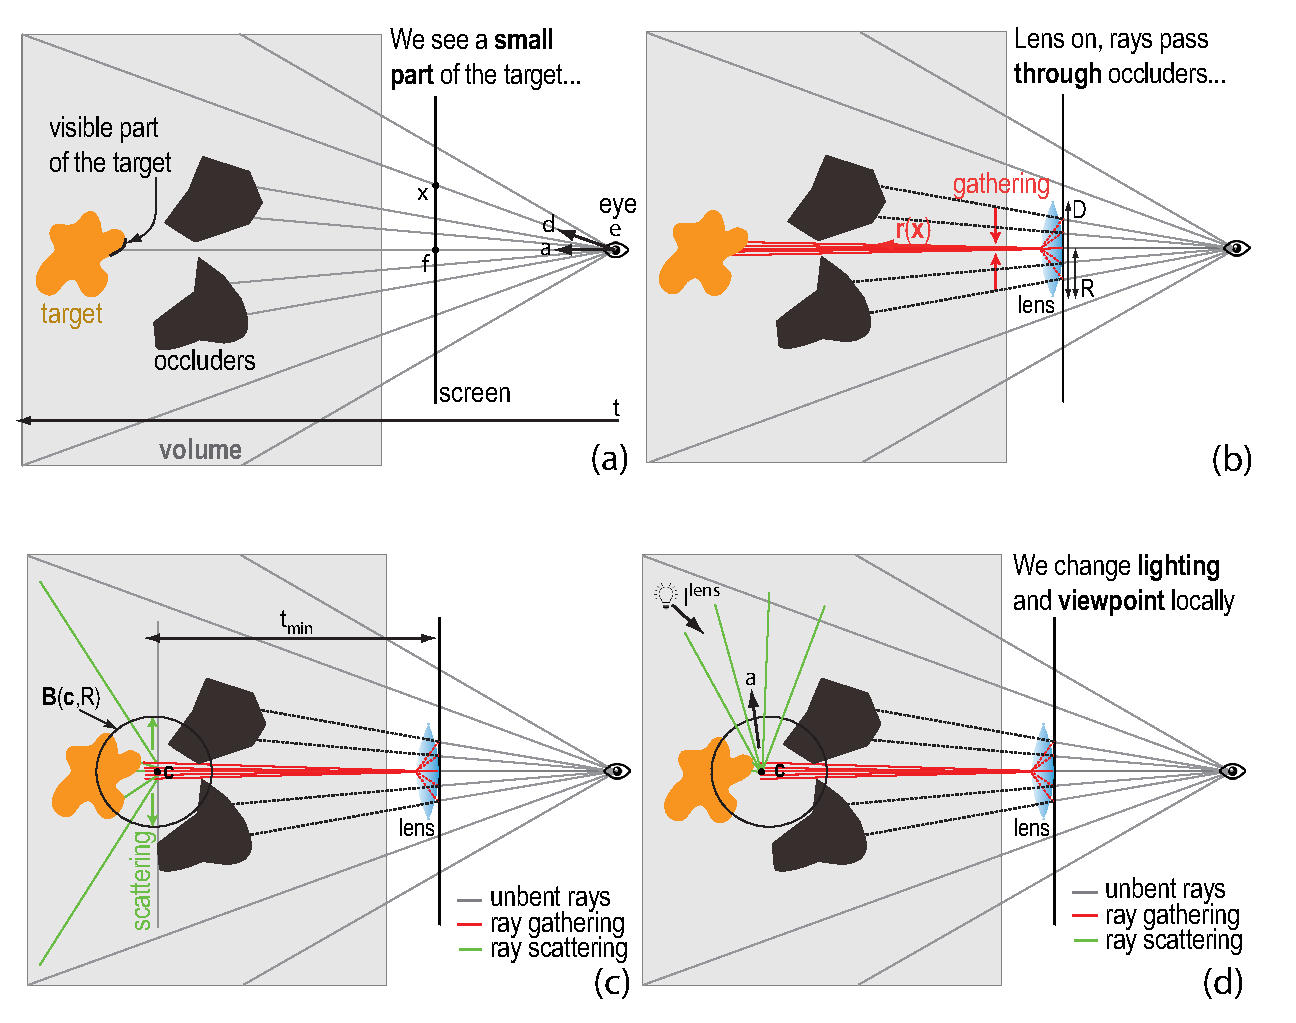
\includegraphics [width=\textwidth]{images/principle.eps}

\caption{Obstruction-free lens working. A target is (mostly) hidden by occluders in front of it. (a) Classic DVR shows a small part of the target. (b) Our lens gathers rays to avoid occluders (\autoref{sec:gathering}). Once close to the target, rays follow again their initial paths. Yet, only a small part of the target is visible. (c) Scattering rays makes the full target visible (\autoref{sec:scattering}). Finally, we adjust the local viewing and lighting directions $\mathbf{a}$, $\mathbf{l}^{lens}$ (\autoref{sec:inter_expl}).}
\label{f:fisheye}

\end{figure}


\section{Principle}
\label{sec:principle}
%
%
Consider the typical DVR algorithm: Given a scalar volume $V \subset \mathbf{R}^3 \rightarrow \mathbf{R}$, each pixel $\mathbf{x} \in I$ in the DVR image $I \subset \mathbf{R}^2$ thereof corresponds to the compositing of sampled data along a ray that passes through $V$ and ends at $\mathbf{x}$. In classical DVR (\autoref{f:fisheye}-a), such rays are defined by the eye position $\mathbf{e}$ and a ray direction unit vector $\mathbf{d} = (\mathbf{x} - \mathbf{e}) / \| \mathbf{x} - \mathbf{e} \|$. Consider now a focus point $\mathbf{f} \in I$ (the lens center) and a lens radius $R > 0$. We modify all rays passing through the lens (focus/0 area $D = \{\mathbf{x} \in I | \| \mathbf{x} - \mathbf{f} \| \leq R\}$ in order to de-occlude, magnify, and emphasize a target object. Our ray behavior is divided into three steps: (1) Provide a clear view of the target by moving closer to it and by pushing occluders aside. (2) Set a wide field-of-view (fisheye) to better see the target. (3) Modify the parameters of the lens, lighting, and opacity TF in real time to better explore the target. These steps are detailed next.

\subsection{Creating an unobstructed view}
\label{sec:gathering}
%
The scenario we address is as follows: Given a volume $V$, users produce a DVR thereof, using whatever suitable TFs and other parameters are applicable. When examining $V$ from various viewpoints, (at least) one viewpoint $(\mathbf{e},\mathbf{d})$ is found from which some intriguing structure is \emph{partially} visible in $I$. We call this structure the \emph{target}. Users next want to quickly and easily unravel the target. For this, we proceed as follows: We first \emph{gather} all rays passing through the lens pixels (focus area $D$) to follow the lens' axis vector $\mathbf{a} = (\mathbf{f} - \mathbf{e}) / \| \mathbf{f} - \mathbf{e} \|$. As explained above, at the location $\mathbf{f}$ of the lens center, we do see an interesting partially occluded target. Hence, by definition, the gathered rays pass \emph{through} occluders to hit this target, otherwise we would not see it. We control gathering by setting the ray direction passing through $\mathbf{x} \in D$ to
%
\begin{equation}
\mathbf{r}(\mathbf{x}) = (1-\alpha) \mathbf{a} + \alpha \mathbf{d},
\label{eqn:gathering}
\end{equation}
%
with $\alpha \in [0,1]$. When $\alpha=0$ (default), all rays follow the lens axis $\mathbf{a}$, thus, can best pass through obstacles. When $\alpha=1$, rays follow a straight path. Changing $\alpha$ with the mouse wheel smoothly navigates between the lens effect, \emph{i.e.} opening up a 'hole' in the volume to see the target, and classical DVR.
%
\subsection{Setting a wide field of view}
\label{sec:scattering}
%
Once the rays pass obstacles (\autoref{sec:gathering}), we want to \emph{scatter} them so as to best sample the target. Consider that this target is at some depth $t_{target}>0$ within $V$. After the rays pass the occluders, but before they hit the target, \emph{i.e.}, travel past a distance $t_{min} < t_{target}$ through $V$, we deflect (scatter) them so as to best sample the target. For this, we set the parametric position of a ray point to
%
\begin{equation}
\mathbf{p}(\mathbf{x}, t) = \mathbf{r}(\mathbf{x})t + \beta (\mathbf{x}-\mathbf{f})(t-t_{min})
\label{eqn:scattering}
\end{equation}
%
for any pixel $\mathbf{x} \in D$ and any $t \geq t_{min}$. Here, $\beta \geq 0$, adjusted via the mouse scroll wheel while pressing the Shift key (\autoref{f:fisheye}-c), controls the ray scattering: Small values magnify a small volume area close to the ray $\mathbf{r}(\mathbf{x})$; larger values sample more of the volume behind the lens. Intuitively, this is as if we moved a magnifying lens to a depth $t_{min}$ inside $V$. Summarizing, after the user finds an interesting but partially occluded target using \emph{standard} DVR, our lens squeezes rays to pass between occluders and next fans them out to explore the target.
%
%


\subsection{Interactive exploration of the target}
\label{sec:inter_expl}
%
To achieve a more effective exploration, we can interactively modify several parameters of the DVR and the lens, as follows.
%
\begin{figure}
\centering

\includegraphics [width=\textwidth]{images/params.eps}

\caption{Changing lighting parameters in the lens. (a) Constant global specular coefficient. (b) Specular coefficient high in the lens and low outside. (c-f) Changing the in-lens light vector yields the effect of a flashlight rotating around the target. The ball icons illustrate the local light vector direction.}
\label{f:params}

\end{figure}
%



\noindent\textbf{Lens radius:} The radius $R$, telling how big is the 'hole' to open up in the volume to see the target, is set via the mouse wheel. The parameters $\alpha$ and $\beta$ (affecting the gathering and scattering of rays respectively) are set by the mouse wheel and modifier keys. The value $t_{min}$ (depth from which scattering starts) is set using the arrow keys.

\noindent\textbf{Lens axis:} Users can rotate the lens axis $\mathbf{a}$ using a virtual trackball activated by the right mouse button. Changing $\mathbf{a}$ effectively samples the target from many viewpoints, allowing the user to look 'around' it to see parts which are not visible from the current viewpoint, but \emph{without} actually changing the viewpoint. This is of high added value, since changing the viewpoint can bring us to a view where the target is fully invisible, so we do not know where precisely to activate the lens anymore. \autoref{f:rotation} shows three such local rotations for the baggage dataset introduced in  \autoref{f:baggage_lens}. From these, we see that the star-shaped target is relatively thick.


\noindent\textbf{Lighting:} We modify the volumetric Phong lighting parameters to better explore the target, as follows. Let $\mathbf{c} = \mathbf{e} + t_{min}\mathbf{a}$ be a point at depth $t_{min}$ along the lens axis, and let $B(\mathbf{c},R)$ be a sphere of radius $R$ around this point (\autoref{f:fisheye}b). We call voxels in this sphere 'in focus', and all other voxels in $V$ 'out of focus'. Let $\phi$ be the specular term coefficient, set to a high value (default: one).
First, for all voxels $\mathbf{x} \in B(\mathbf{c},R)$, we use a specular coefficient $\phi(\mathbf{x}) = \phi (1-d)$, where $d=\|\mathbf{x}-\mathbf{c}\|/R$. For all voxels outside $B(\mathbf{c},R)$, we use $\phi(\mathbf{x}) = 0$. Hence, voxels close to the focus point $\mathbf{c}$ appear highly specular; further away from $\mathbf{c}$, voxels get less specular, and voxels out of focus are purely diffuse. Secondly, we allow the user to locally rotate the light vector using the same trackball mechanism as for the lens axis rotation. Let $\mathbf{l}^{lens}$ be this vector, and let $\mathbf{l}^{global}$ be the global light vector used by standard DVR. For all voxels in focus, we use a light vector $\mathbf{l}(\mathbf{x}) = (1 - d)\mathbf{l}^{lens} + d\mathbf{l}^{global}$. As the user rotates $\mathbf{l}^{lens}$, the light direction will visibly change in the middle of the lens, stay constant outside it, and smoothly change in between.


The above two mechanisms combined yield the effect of a moving flashlight turning around a shiny target embedded in a constantly-lit diffuse scene. \autoref{f:params} shows these mechanisms for a chest CT dataset containing a deeply buried tumor (the dataset and use-case are described in detail in \autoref{sec:chest}). We see how turning the light highlights small-scale details on the target surface (tumor) without changing the viewpoint or lens location. Moreover, the high specularity in the lens attracts the user's attention to this area; the diffuse lighting outside the lens put less emphasis on the context area. 


\noindent\textbf{Opacity:} We modify the opacity transfer function along a similar idea as for lighting ( \autoref{fig:tf}). Let $TF_{o}^{global} : \mathbf{R} \rightarrow [0,1]$ be the user-chosen opacity function used globally for the volume. Let $\Gamma$ be a Gaussian pulse of unit height centered at the average density value $\bar{\rho}$ in $B(\mathbf{c},R)$ and with standard deviation $\sigma$. We estimate $\bar{\rho}$ and $\sigma$ by considering the density $\rho$ at 150 points randomly sampled inside $B(\mathbf{c},R)$. Higher values for the sample count yield visually very similar results for our tested volumes of up to $500^3$ voxels, while requiring (slightly) more computation costs. Then, for voxels in $B(\mathbf{c},R)$, we use an effective opacity transfer function $TF_o = TF_{o}^{global} + (1-d) \Gamma$. For voxels outside $B$, we use $TF_{o}^{global}$ (standard DVR).
This is useful when the user sets $TF_{o}^{global}$ to make most out-of-lens voxels relatively transparent. In that case, $TF_o$ will still make voxels in $B$ opaque, thus allowing to see the in-focus structures better. \autoref{f:params} has been generated this way.


%ALEX: This phrase was indeed confusing, I don't know what we wanted to say with it: 
%We see here how the tumor in the lens has the same opacity as the muscle tissue outside the lens, even though the two have nearly identical densities.

\begin{figure}
\centering
\includegraphics[width=0.95\textwidth]{images/tf.eps}

\caption{Construction of local transfer function $TF_{o}$. See \autoref{sec:inter_expl}.}

\label{fig:tf}
\end{figure}


\subsection{Smooth transitions}
\label{continuity} 
%
If we bend rays passing through the lens pixels $D$ (\autoref{eqn:gathering} and \autoref{eqn:scattering}) and trace rays starting at pixels in $I \setminus D$ as straight lines, discontinuities appear at the lens borders. We solve this as follows. Let $\mathbf{p}(\mathbf{x},t)$ be the voxels along a lens ray starting at screen pixel $\mathbf{x}$, as computed by  \autoref{eqn:scattering}. Let $\mathbf{p}^{line}(\mathbf{x},t)$ be the voxels along a straight-line ray starting at $\mathbf{x}$, \emph{i.e.}, computed using $\alpha=1$ and $\beta=0$ in  \autoref{eqn:gathering} and \autoref{eqn:scattering} respectively. For every value $t$ along every such ray, we compute the interpolated ray $\bar{\mathbf{p}}(\mathbf{x},t) = (1-f(d))\mathbf{p}(\mathbf{x},t) + f(d)\mathbf{p}^{line}(\mathbf{x},t)$, where $d$ is the distance of $\mathbf{x}$ to the lens axis (normalized to unit by dividing it by $R$) and $f : [0,1] \rightarrow [0,1]$ is an interpolation function. Next, we use the rays $\bar{\mathbf{p}}(\mathbf{x},t)$ to compute the DVR by standard composition. This way, rays effectively vary smoothly from their bent versions (close to the lens axis) to straight lines (outside the lens). Setting $f(d) = d^2$ keeps the interpolation transitions close to the lens border, so most of the lens is dedicated to show the desired fisheye effect.

\begin{figure}
\centering
\includegraphics [width=0.95\textwidth]{images/rotation.eps}

\caption{Performing local rotations in the lens allows better seeing the shape and thickness of the partially occluded target object (ninja star).}
\label{f:rotation}

\end{figure}

Separately, we use a slow-in/slow-out animation\,\cite{Dragicevic:2011:TDA:1978942.1979233} to introduce the lens effect. When activating the lens, we vary $\alpha$ and $\beta$ from their defaults ($\alpha=1$, $\beta=0$, \emph{i.e.} straight-line classical DVR) to their actual user-set values, compute the volume rendering on-the-fly, and display the resulting images. The effect resembles gradually opening a hole in the volume -- see the associated video. The speed increase at the start of the animation helps one to quickly see what is revealed in the lens; the decreasing speed at the end helps seeing where the pushed-away occluders actually go. This also gives some semantic to the moving shapes, allowing one to interpret the motion as a magnification of a target, and to keep the focus on visual entities during this transition. When deactivating the lens, we play back the animation in the opposite sense, which suggests closing the opened hole in the volume.

\section{Implementation}
\label{sec:implem}
%
We implemented our occlusion-free lens by modifying a standard DVR ray caster, publicly available in NVIDIA CUDA's SDK\,\cite{cudasdk}. We modified this ray caster to incorporate the new ray definition (\autoref{eqn:gathering} and \autoref{eqn:scattering}), the lens effect, and the local per-voxel Phong lighting parameters, all controlled via keyboard and mouse. On a PC with 16 GB RAM and a GeForce GTX TITAN X card, we achieve 15 frames per second for volumes up to $512^3$ voxels at a $1900 \times 1200$ pixels screen resolution. All in all, adding our lens to an existing ray caster should pose no significant implementation problems.

\section{Application Scenarios}
\label{sec:scenarios}
%
We next demonstrate our obstruction-free lens via five use-cases considering scalar density volumes from baggage inspection, 3D flow simulation, radiology, air traffic planning, and diffusion tensor imaging.

\subsection{Baggage inspection: An unusual blunt object}
\label{sec:baggage}
%
In airports, security agents deal with volumetric data exploration during baggage inspections. While automatic systems can detect densities of harmful substances such as C-4, TNT, and nitroglycerin, or prohibited articles (threats) like classical firearms and knives, unusual threats are hard to find. Four main concealment strategies exist\,\cite{7819413}:
\begin{itemize}
\item \textbf{Superposition}: A threat may be sheltered among dense materials. While possible to see through such a 'shield' using high penetration (enhanced X-ray power) or image processing (contrast improvement), such techniques are not universally available and also require fine-tuning many parameters, which slows down inspection.


\item \textbf{Location}: Objects located in the corners, edges, or in the luggage's frame are very hard to spot.


\item \textbf{Dissociation}: One can conceal a threat by spreading its parts in the luggage, \emph{e.g}, by disassembling a weapon and scattering its parts.

\item \textbf{Lure}: A minor threat (lure) like small scissors is clearly visible and catch the security agent's attention who can miss the real threat.

\end{itemize}


\begin{figure}
\centering
\includegraphics [width=\textwidth]{images/shuriken.eps}

\caption{(a-c) A baggage scan is viewed from different angles. In view (c), a suspicious sharp object is spotted between a set of mugs. (d-f) Filtering densities using a classical 1D opacity transfer function removes progressively more of the occluders (mugs), but also the target. (g) The user applies the lens on the target object (double-click). An animation starts opening the lens, rays are gathered to pass through occluders. Halfway the animation, the object is magnified, but only the area close to the lens is visible. (h) The fish-eye field of view at the end of the animation scatters rays to fully show the target. (i) The lens is increased to magnify the target (mouse scroll).}
\label{f:baggage_lens}
\end{figure}


Baggage labeled as suspicious by human inspection or automated scan heuristics must be checked by human agents. Besides time-consuming physical unpacking, one can use 'virtual unpacking' tools that segment the 3D scan by a density-based confidence measure and next move the segmented objects away by animation to reduce occlusion\,\cite{Li:2012:LVV:2425296.2425325}. Such systems have been patented and used in production\,\cite{patent}. However, when the automatic segmentation is not optimal, the user must manually change its parameters, repeat the segmentation and animation, which goes back to being time-consuming.

Consider the baggage scan in \autoref{f:baggage_lens} ($283 \times 189 \times 344$ voxels, dataset obtained from an actual airport scan). Automatic baggage inspection systems will not detect anything suspect here. However, while visually exploring this baggage from different angles (\autoref{f:baggage_lens}a-c), we see an object hidden between a set of mugs. To reduce occlusion, a common solution in baggage inspection is to filter materials by density in order to show or hide subsets of the volume. However, for our dataset, the suspect target has almost the same density as the surrounding mugs, so removing the latter also removes the target (\autoref{f:baggage_lens}d-f). Using the obstruction-free fish-eye lens helps here: Clicking on the sharp detail visible in \autoref{f:baggage_lens}c first gathers rays so they pass through the low-density zone between the mugs (\autoref{f:baggage_lens}f). The animation that opens the lens 
(\autoref{f:baggage_lens}e-g) reveals an unobstructed view of the target. However, this shows only a small part of the target. Scattering rays next fully reveals the target (\autoref{f:baggage_lens}h). Adjusting the lens size shows a more detailed view of the target (\autoref{f:baggage_lens}i). Next, locally turning the viewpoint around the target (\autoref{f:rotation}) allows the agent to decide that the target is a shuriken (Japanese ninja star weapon). Since the object is very thick and blunt (see \autoref{f:rotation}), it is not an actual weapon, thus not a threat.

We evaluated our lens for this use-case by a user study. Eight airport security specialists were recruited (ages 23 to 43; experience in baggage scanning 8 months to 20 years; average familiarity with 3D tools, none considering him/herself an expert, see \autoref{fig:questanswers}).


All attended a 20-minute global demo of the lens operation. Next, they were given each a personal training session for using the tool (5 minutes), in which they were instructed on the mouse and keyboard controls. After this, they were asked to work in pairs to examine the above-mentioned baggage CT dataset to form a decision on the nature of the ninja star possible threat (20 minutes of tool usage per person, after which the pair was changed). The idea behind this is that one person operates the tool while the other poses questions or suggest explorations, much like typical airport security operators work with a scanner. In the end, they all separately filled in a web questionnaire covering several questions and also provided open feedback (questionnaire available in the \autoref{AppendixA}). 

\autoref{fig:questanswers} shows the answers. The first question-set (S1) regarded how easy-to-use, generally effective, and effective \emph{vs} other known tools our lens is for \emph{untargeted} inspection, \emph{i.e.}, when no suspect target is partially visible. Here and next, other tools denote classical 2D X-ray or 3D CT scans used in baggage scanning that the subjects know. As \autoref{fig:questanswers}c-e shows, 
the answers (on a 5-point Likert scale) were predominantly positive: The tool is easy to use, is useful, and is actually more useful than known tools for untargeted exploration. The second question-set (S2) regarded how good our tool is to examine \emph{specific} targets which are partially visible. Here again, the answers were predominantly positive (\autoref{fig:questanswers}f-h). The main appreciated features of our tool are listed in \autoref{fig:questanswers}i.


\begin{figure}
\centering
\includegraphics [width=0.5\textwidth]{images/questanswers.eps}
\caption{Evaluation of lens-based baggage inspection (\autoref{sec:baggage}).}

\label{fig:questanswers}
\end{figure}

We next summarize the received open feedback. According to the subjects, our tool can provide them a better perception of the items inside the baggage as compared to the classical 2D single-viewpoint X-ray machinery they routinely use. Quotes from the open feedback: ''clear added-value compared to all systems I know''; ''this tool is a real gain for examining luggage with uniform and/or high densities''; ''definitely better than known tools for examining threats I am not familiar with / I have not seen before''. However, our tool should not be used for the typical carry-on baggage inspection which has a very small allowed inspection time (15 to 20 seconds). Our tool is much more interesting for inspecting checked-in baggage, where inspection time-windows are up to 3 minutes. The perceived added value for this use-case is also higher: Opening up checked-in baggage for manual inspection is much more complicated and time-consuming than for carry-on baggage. Moreover, the only system for inspecting checked-in baggage that the subjects knew of is a scanner that aims to \emph{automatically} detect threats via X-ray imagery; this system suffers from false positives, so a manual examination tool like ours could quickly eliminate such false positives, and thus the delays of opening up checked-in baggage. Finally, several subjects suggested that adding a function to display a classical 2D slice view (activated by a key press and aligned with the focal point) would be useful since this would show additional detail.


\subsection{Fluid flow: A deep-buried spherical vortex}
\label{sec:flow}
%
%
Flow visualization using streamlines has a long history\,\cite{brambilla2012illustrative,merzkirch2012flow}. For 3D datasets, a key challenge is to balance the streamline density. Low values allow seeing inner regions in the data but can subsample (miss) patterns. High values show more data but create too much occlusion. We next show how our lens can be used to alleviate problems in the latter case. The dataset\,\cite{griebel2004flow} captures the simulation of water flow in a basin computed on a grid of $128 \times 85 \times 42$ cells using 4595 streamlines with 183K sample points traced by pseudo-random seeding. We convert this set of 3D curves (polylines) to a scalar volume by using GPU-accelerated kernel density estimation (KDE)\,\cite{lhuillier2017ffteb}. Similar techniques have been used to compute density maps of 2D trail-sets\,\cite{hurter2012graph,cubu,hurter2015image}. 

We first explore the density volume ($500^3$ voxels) using standard DVR (\autoref{f:stream_lens}). Note that, given KDE's smoothing effect, streamlines appear as finite-thickness tubes rather than pixel-thin curves. After turning the viewpoint a bit, we notice a dense spherical item deep in the data (\autoref{f:stream_lens}a). To see its shape better, we increase opacity; however, this immediately increases occlusion so the item becomes invisible. Conversely, decreasing opacity to reduce occlusion makes the item almost transparent. Our lens solves the problem: In the initial view (\autoref{f:stream_lens}a), we point at the target and turn on the lens. This pushes away the occluding stream bundles, and shows that our item is a set of densely-packed, low-speed, tightly-turning streamlines that create a ball-like vortex (\autoref{f:stream_lens}b). 
To make sure our target is spherical, we view it in the lens from different directions, by interactively changing the ray directions in the lens (\autoref{f:stream_lens}c). Finally, we can close the lens but keep the target magnified (\autoref{f:stream_lens}d).
Finding the details of this vortex cannot be done using standard DVR. Interestingly, this vortex has also not been discovered by any of the visualization techniques that used this dataset (according to our knowledge) \,\cite{telea_vis_99,griebel2004flow,ddh,lhuillier2017ffteb}. 

\begin{figure}
\centering
\includegraphics [width=\textwidth]{images/stream_lens.eps}

\caption{Flow volume exploration with two different opacity transfer functions (top and bottom rows). In viewpoint (a), we notice a small high-density spherical item. (b) We apply the lens at that location (double click). (c) The directions of rays in the lens are changed to see the whole target in the lens (right click + mouse drag change direction). (d) The lens is gradually closed while keeping the focus area magnified (shift + scroll).}

\label{f:stream_lens}
\end{figure}

\subsection{Chest scan: A hard to see tumor}
\label{sec:chest}
%
In our third use-case, we consider a contrast chest CT scan ($512 \times 512 \times 110$ voxels) of an elderly patient with a sizeable lung tumor. The tumor was detected in a CT scan performed after the patient reported acute chest pain. Typical examination of these scans by the pulmonologist and radiologist in charge involves slice-based views. \autoref{f:slicer}a-c and \autoref{f:slicer}d-f show two such slice sets (axial, coronal, and sagittal views), produced using typical lung, respectively mediastinal, contrast presets.

 Although the tumor is visible in all these views, its exact shape, morphology, and connection to the lung walls are hard to assess. Finding such details on the tumor is essential, explained the doctors in charge, to determine the TNM score\,\cite{brierley} and also planning treatment. Using standard DVR makes the tumor and its 3D position partially visible (\autoref{f:slicer}f). Yet, occlusion from the rib cage and other tissues is still present. Using both TF presets and manually changing the TFs in the 3D Slicer tool\,\cite{slicer} used to create the DVR could not help de-occluding the tumor without making it partly transparent.
 
  The slice images in \autoref{f:slicer}a-f confirm this by showing that the gray values for the tumor and surrounding skin-and-muscle tissue are very similar. This is due to the fact that the tumor had grown rapidly and started necrotizing, which filled it with fluids, making its density very similar to that of the obstructing (skin and muscle) tissue, explained the pulmonologist. Hence, one cannot remove such occluding tissue in a classical DVR setting by opacity TF manipulation without also removing the tumor. This makes examining this specific tumor harder than for regular cases.

\begin{figure}
\centering
\includegraphics [width=\textwidth]{images/slicer.eps}
\caption{Lung tumor visualization using slices (a-c) and standard DVR (d). Annotations are manually added by the examiner to delineate the tumor location. Images constructed using the 3D Slicer tool\,\cite{slicer}.}
\label{f:slicer}
\end{figure}

We next used our lens to examine the tumor. \autoref{f:params} shows several sample snapshots. We see that the tumor is significantly more visible when using the lens than when using standard DVR (\autoref{f:slicer}d), both in terms of removing the occluding tissue and in terms of the tumor's opacity -- compare the inset in \autoref{f:slicer}d with the images in \autoref{f:params}. Secondly, relighting the tumor from various directions allows one to see small-scale morphological details such as the tumor's surface shape and its connection via protuberances and veins with the lung walls.

We asked the two medical specialists (pulmonologist and radiologist) in charge to state the potential advantages and/or limitations of our lens as compared to standard slicing and DVR techniques, after a 20-minute usage of the tool. 
Both specialists have over 10 years of medical experience in treating lung cancer, and routinely use several slicing and DVR tools. They work in a private hospital in Belgium and are not actively associated with medical imaging research. Our identities were hidden from them during the lens evaluation. The provided input can be summarized as follows: The occlusion-free lens is definitely easier and faster to use than classical DVR and/or slicing techniques. It is especially more effective than these to get a quick, first impression of a deep buried anatomical detail. Changing the lens' parameters by direct interaction is as simple as changing window/level functions in a typical slice-based tool, and is definitely simpler than tuning typical DVR parameters to obtain similar results. This 'entices' the user to explore, which is a good aspect. The fact that the lens minimizes viewpoint change (volume rotation), \emph{i.e.}, after a suitable viewpoint was found from which a (small) part of the target is visible, one doesn't need to change this viewpoint, is a strong feature, as 3D viewpoint changes are disruptive and cost time. This is important in a cost-aware environment where specialists have very limited time (about 20 minutes) to assess a CT scan. However, the lens should not \emph{replace} classical slice-based exploration, which shows small-scale details better. In the context of the current dataset (\autoref{f:slicer}), the lens was useful to both confirm the TNM score (T3 grade tumor, 6.5 cm in size) found via the 2D slices, but much more so for understanding how and where the tumor is connected to surrounding tissue, which is very hard to do using only 2D slices.

\begin{figure}
\centering
\includegraphics [width=\textwidth]{images/aircraft.pdf}

\caption{Visualizing one day of aircraft trajectories over France\,\cite{hurter2009fromdady}. (a) Overview of all trails. (b) Zoom, filtering, and color mapping techniques are used to highlight an outlier trajectory of an aircraft performing an eight-shaped loop. Revealing this outlier costs significant user effort.}
\label{f:fromdady}

\end{figure}


\subsection{Aircraft trajectories: Outliers in the French sky}
\label{sec:atc}
%
%
We next consider a task from air traffic planning -- detecting and studying outliers in large-scale datasets containing tens of thousands of 3D (latitude, longitude, height) trails of aircraft over a given spatio-temporal region\,\cite{hurter2014interactive}. Such datasets are typically viewed using 2D (latitude, longitude) plots where opacity encodes the spatial density of flights -- see \autoref{f:fromdady}a, which shows one day of recorded aircraft trajectories over the French airspace. \autoref{f:fromdady}(b) shows a detail zoom-in, where we can see an abnormal -- that is, far from straight or slightly curved -- aircraft trail: A tanker aircraft performed an eight-shaped loop as it was waiting to refuel other aircraft. Revealing such patterns using 2D techniques, \emph{e.g.} \cite{hurter2009fromdady}, is very hard. In particular, it is hard to de-occlude these patterns from the overall context of criss-crossing aircraft trails, even when one knows their 2D spatial location.

Our lens can help with this task, as follows. We first convert the set of 3D trails to a $500^3$ density volume, using KDE as for the streamline use-case (\autoref{sec:flow}). Examining this volume via standard DVR shows an outlier trail at some point in space, see curved patterns in \autoref{f:aircraft_lens}a. Activating the lens on this area and interactively tuning the target depth $t_{min}$ (since we don't know the trail's height) beings the outlier trajectory in focus and pushes away occluding trails (\autoref{f:aircraft_lens}a). Like in the other examples presented so far, we can quickly change the magnification factor and view direction to better study this trail in context (\autoref{f:aircraft_lens}b-d). From these images, we easily see that the outlier trail has an eight shape. Revealing this outlier trail using standard 2D visualization techniques\,\cite{hurter2009fromdady} costs several minutes. Doing the same using our lens costs under one minute. Also, comparing \autoref{f:fromdady}b and \autoref{f:aircraft_lens}b-d, we argue that the eight-shape of the outlier trail is much more prominent, and thus recognizable, in the latter images (made using our lens) than in the former ones. Last but not least, the 3D DVR approach that our lens enhances explicitly encodes flight height information, so our lens can use it by interactively tuning the depth value $t_{min}$ where the lens is focused. This cannot be done with 2D techniques which ignore the depth dimension.

We validated our findings with an air traffic data scientist with more than 10-year experience in air traffic control and planning. She confirmed that this specific eight-shape trail in \autoref{f:fromdady}(b) is an actual aircraft which performed waiting loops and acted as a fuel supplier for military aircraft. Other comments included the following: Compared to standard 2D visualization techniques, our tool makes detecting outliers easy since there is no need for complex manipulation to reveal such outlier trails. Also, the user does not have to deal with color and alpha mapping parameter-tuning to make specific outliers emerge. Separately, trail visualization easily creates many occlusions leading to either fully opaque areas or too much local overlap, which both hinder seeing and examining specific trails. Our lens does help such cases by distorting the space to locally remove such occlusions. All in all, in the studied dataset (\autoref{f:fromdady}), the lens was specifically useful since, for high transparency, one would not detect the outlier trail, while for low transparency, one would get a hint of the outlier's existence, but not see it in detail due to too much occlusion; the lens allows using low transparency, but removes the clutter caused by it to reveal the outlier.


\begin{figure}
\centering
\includegraphics [width= \textwidth]{images/aircraft_lens.pdf}
\caption{Inspecting an abnormal aircraft trail. (a) The abnormal trail is spotted in an all-trails view as it is highly curved while all other trails are relatively straight. Activating the lens at the outlier location (b) and changing the magnification factor (c) reveals the trail's eight-shape. (d) Rotating the viewpoint provides spatial insight on the embedding of the outlier in the surrounding trails.}
\label{f:aircraft_lens}
\end{figure}
%

\subsection{Brain fibers: Uncluttering the bridge}
\label{sec:dti}
%
Our last use-case considers the exploration of fiber tracts visualized as streamlines of the major eigenvector of a diffusion tensor imaging (DTI) field. Such datasets have a spatially complex structure which makes them hard to explore\,\cite{assaf08}. In particular, fiber tracts are spread volumetrically over the entire extent of the brain, and create tangled patterns inside which it is hard to see much. DVR techniques are often used to render such tracts, one of the advantages being that close fibers get visually 'merged' to reveal spatially coherent structures, an effect which is not possible when fibers are rendered as polylines. However, DVR methods also create more occlusion, thus difficulties in seeing structures deep within the volume.

We consider an $128 \times 128 \times 51$ DTI volume (same dataset as in\,\cite{everts15}). We traced 150352 fibers seeded in, and going over, regions of high fractional anisotropy in this volume. We filtered out fibers shorter than 2mm, yielding a total of 120593 fibers to display (6.4M sample points). Next, we converted this fiber-set to a $512^3$ density volume, using KDE with a 3D isotropic kernel of radius 15 voxels, like for the streamline use-case (\autoref{sec:flow}). \autoref{fig:dti}a shows the result, rendered with DVR, with opacity function mapping the fiber density. While terminal fibers are well visible, we cannot see anything inside the volume. Activating the lens in the middle of the volume opens a hole through which a small part of the \emph{corpus callosum}, the fiber bundle wrapping the bridge that connects the two hemispheres, becomes visible. By slightly decreasing opacity (\autoref{fig:dti}c), the \emph{corpus callosum} gets clearly visible, appearing as a compact structure, due to the KDE blending of neighbor fibers. Obtaining such a view of the \emph{corpus callosum} only using DVR would be very hard, since transfer functions would either render separated (non-merged) fibers, or else make the fibers surrounding the structure of interest too thick and occluding. 

This scenario has the main difference compared to all previous ones. In all earlier cases, the standard DVR of the data (that is, without the lens) showed us a partial small cue of the structure of interest within the volume, and we used the screen-space location of this structure as the focus point where to activate the lens. In this last scenario, there is no point in the original DVR image (\autoref{fig:dti}a) from which the \emph{corpus callosum} is even partially visible, due to the high opacity given by the used transfer function. Hence, the user can activate the lens at \emph{any} desired point to peek inside, and towards the center of, the volume. Given the nature of the data, the structure of interest is quite easily visible from most such viewpoints (see lens inset in \autoref{fig:dti}b). Once its presence is revealed, the user can next adjust the viewpoint and/or the opacity transfer function to get an optimal view on the target, such as the one shown in \autoref{fig:dti}c. Summarizing, we can use our lens also in cases when no partial view of a target is available. 

\begin{figure}
\centering
\includegraphics [width=\textwidth]{images/dti.eps}
\caption{Revealing the \emph{corpus callosum} in a DVR of a set of DTI tracts.}
\label{fig:dti}
\end{figure}

%
\section{Discussion}
\label{sec:discussion}
%
%
Several points of our lens proposal are worth discussing, as follows.

\vspace{0.15cm}
\noindent\textbf{Lens activation:} Our lens can support two types of explorations. First, when the user perceives a \emph{part} of a target of interest in a classical DVR image, the lens can be used to reveal the target in full detail. This \emph{directed} exploration supports the task `show me more information about \emph{this} item'. The use-cases in \autoref{sec:baggage}-\autoref{sec:atc} are of this type. Secondly, the user can open up a DVR volume at a 2D location from which no partial detail is visible. This is useful when we know that there \emph{is} an interesting target buried in the volume even without seeing it (\emph{corpus callosum} use-case in \autoref{sec:dti}), thus supports the task `show me the data I \emph{know} it is somewhere in there', or for free exploration to find unknown patterns in a volume, \emph{i.e.} for the task `show me what this volume \emph{may} hide in it'. In the first exploration type (target not fully occluded), our lens is simple and rapid to use -- point, click, and optionally rotate light or viewpoint. In the second exploration type (target fully occluded or not even sure whether an interesting target exists in the data), the lens is equally simple to use, but several tries to select a suitable focus point and lens depth are needed.

\vspace{0.15cm}
\noindent\textbf{Lens shape:} Occluders are pushed away, and deformed, isotropically (\autoref{sec:scattering}, \autoref{continuity}). This simple lens model requires a single parameter, the lens radius $R$, which makes its usage easy. The deformations evolve smoothly from the lens center (maximal) to outside the lens (no deformation), see \autoref{continuity}, which effectively blends the local (in lens) focus with the global (out of lens) context (R3). However, this strongly compresses the deformed occluders close to the lens border, making them hardly visible when the lens is fully active. A possible refinement would be to reduce the deformation of the pushed-away occluders while still pushing them away, thereby improving the F+C effect (R3). However, this would occlude areas outside the lens, basically moving occlusion from \emph{inside} the lens to \emph{outside} and close to it. Finding an optimal balance between minimal deformation (so one can recognize the pushed-away occluders) and minimal clutter (so these occluders do not destroy the lens context) is a topic for future work. Separately, deformed rays may intersect with straight rays, thereby sampling the same voxel(s) to different image pixels. We did not observe in our usage any artifacts that can be ascribed to this issue, nor did the other users of our tool. This can be explained by the fact that such ray intersections are relatively few and we use a compositing transfer function, akin to a low-pass filter.

\vspace{0.15cm}
\noindent\textbf{Parameter setting:} Our lens depends on several parameters: the 2D lens center $\mathbf{f}$, lens radius $R$, lens axis direction $\mathbf{a}$, local light direction $\mathbf{l}^{lens}$, scattering start-distance $t_{min}$, and gathering and scattering parameters $\alpha$ and $\beta$. All these parameters are controlled via a mouse-driven virtual trackball, key modifiers, and the arrow keys (\autoref{sec:principle}). As the lens works at 15 frames per second, the user can quickly tune the parameters and see their effect (R1). Moreover, all parameters start with good preset values (\autoref{sec:principle}). A possible refinement would be to pre-segment the target, based on user-given values for $\mathbf{f}$, $R$, and $t_{min}$, thereby determining $\beta$ automatically. However, we believe that manual control of the scattering $\beta$ is important to allow users to choose their most suitable field-of-view angle. In fact, this flexibility allows a better exploration of the local context (R2).

\vspace{0.15cm}
\noindent\textbf{Implementation:} We implement our lens by modifying the ray trajectories constructed in the inner loop (per-pixel raycasting) of a public DVR raycaster\,\cite{cudasdk}. Apart from this, we change the per-voxel lighting and transfer function based on the voxel location in the lens and the parameters given by user interaction (\autoref{sec:inter_expl}). Such changes are limited and easily applicable to any (parallel) raycaster.

\vspace{0.15cm}
\noindent\textbf{Limitations:} As explained, de-occluding a target requires either a small fragment thereof to be visible (if so, de-occlusion is very simple and fast), or requires the user to choose the lens focus and target depth based on other insights (which, as explained, requires more trial-and-error). At a higher level, many lens mechanisms exist in the literature, as discussed in \autoref{sec:requirements}. While we have argued that, to our knowledge, none of them simultaneously supports requirements R1,$\ldots$,R4, comparing such mechanisms with our lens for specific use-cases and datasets is an important test for the \emph{end-to-end} effectiveness of our proposal. We have not covered this point as obtaining (or replicating)  implementations of such lenses is very challenging. This remains an important open point for future work -- both for our proposal but also for all other volumetric lens proposals in the literature. In particular, none of the techniques in \autoref{tab:methods} were compared side-by-side against other techniques. We have performed three user evaluations involving specialists in airport baggage security (\autoref{sec:baggage}), pulmonology (\autoref{sec:chest}), and air traffic control (\autoref{sec:atc}). In all cases, users were not involved in this work, nor with other work of the authors. However, the set-up of these evaluations stays at the level of formative user experiments. To confirm and refine the obtained (positive) findings, more formal user studies are needed, which we plan to cover next.

\section{Conclusions}
\label{sec:conclusions}
%
In this paper, we presented a new fish-eye-like context-and-focus lens that addresses the occlusion problems inherent in scalar volume rendering. The principle of our lens consists in first gathering (squeezing) rays so that they easily pass through occluding densities (given a user-specified opacity transfer function) and next scattering (fanning out) rays to best sample the target of interest. Our lens can be directly applied to any DVR raycaster and scalar volume dataset. Its main constraint is that the user should be able to find a viewpoint from which the target of interest, deep buried in the data, is at least slightly visible. We also present several modifications of the local rendering parameters within the lens (view direction, lighting parameters, opacity transfer function) that aim to both better separate the focus (lens) from the context (volume) and also allow more detailed examining of the target. Our lens is easy to use -- all its parameters are controlled via direct mouse-and-keyboard interaction -- and can be efficiently implemented atop of a standard GPU ray caster. Our lens is especially useful for highlighting structures of interest which are both deeply embedded in volumetric data and cannot be revealed by standard transfer function manipulations due to similar densities in the occluders and target. We demonstrate these points using five use-cases involving datasets from baggage detection, fluid visualization, air traffic control, and chest radiology, and DTI fiber tracts.

Several improvements to our proposal are possible, as follows. First and foremost, heuristics can be sought to link all our free parameters (lens size, focus depth, interpolation between focus and context) directly to the volume data, so the user interaction is minimized and therefore exploration efficiency is increased. Secondly, our lens could be extended to different types of volumetric datasets, such as multivariate (vector, tensor) fields. Last but not least, a formal wider-scale evaluation of how the lens addresses more specific tasks, and how it compares to existing tools for these tasks, such as other lens types, is a goal we aim to pursue next.
\chapter{Volume rendering on mobile devices (Virtual Reality, Augmented Reality, Mixed Reality) }
\label{mixedReality}

This chapter presents the research I have started at the end of this thesis. 
We address the volume rendering challenges on mobile devices (Virtual reality, augmented reality, and mixed reality). Mobile devices are getting more and more popular across the population. Although their technical specifications can be totally different from one device to another, they are all becoming more powerful int terms of memory, CPU, GPU, and features.

\section{Introduction}

First of all, let us define and be more following terms: virtual reality, augmented reality, and mixed reality.

\par \textbf{ Virtual Reality (VR)} immerses users in a fully artificial digital environment. In fact, This technology immerses users in a completely virtual environment that is generated by a computer. The most advanced VR experiences even provide freedom of movement – users can move in a digital environment and hear sounds. Moreover, special hand controllers can be used to enhance  virtual reality experiences.\newline
You need to wear a special VR headset to experience virtual reality. Most VR headsets are connected to a computer (Oculus Rift) or a gaming console (PlayStation VR) but there are standalone devices (Google Cardboard is among the most popular) as well. Most standalone VR headsets work in combination with smartphones: the user insert a smartphone into a headset, then wear this headset, and immerse in the virtual reality.

\par \textbf{Augmented Reality (AR)} allows users to see and interact with the real world while digital content is added to it. As a popular example, we can think of Pokemon Go which causes millions of people all over the world have been rushing with their smartphones in search for small virtual creatures. That is the most pertinent example of augmented reality. \newline
If you own a modern smartphone, you can easily download an AR app and try this technology. There is a different way to experience augmented reality, though  with special AR headsets, such as Google Glass, where digital content is displayed on a tiny screen in front of a user's eye.

\par \textbf{Mixed Reality (MR)} is the most recent development in reality technologies that sometimes causes confusion, primarily because different experiences are called so. Without going too deep into science, let us look at two forms of reality technologies that are referred to as mixed reality (As I have mentioned just one of them at the very beginning):

\begin{itemize}

\item \textbf{ Mixed reality that starts with the real world }– virtual objects are not just overlaid on the real world but can interact with it. In this case, a user remains in the real-world environment while digital content is added to it; moreover, a user can interact with virtual objects. This form of mixed reality can be considered an advanced form of AR.

\item  \textbf{Mixed reality that starts with the virtual world} – the digital environment is anchored to and replaces the real world. In this case, a user is fully immersed in the virtual environment while the real world is blocked out. It almost looks like virtual reality. In fact it does, but the digital objects overlap the real ones whereas in conventional VR the virtual environment is not connected to the real world around a user. To experience this form of mixed reality, you can wear Windows mixed reality headsets. 
\end{itemize}

\section{Stereoscopic 3D}

Stereoscopic 3D is used in virtual reality and  mixed reality systems.
This  is a technique that produces an illusion of depth in a moving image by displaying two slightly different images to the right and left eye of the observer . This ability is based on the characteristics of the human visual system. The eyes, being positioned horizontally in the head, receive two views of the visual scene - one for the left-eye and another for the right-eye. The views overlap but differ slightly since they originate from two distinct perspectives. The visual system interprets and processes the information gathered from the two images to produce stereoscopic depth. The binocular system is very good at coordinating the movement of the eyes, which move constantly even during fixation. From a functional point of view, the images of both eyes fall on the fovea when fixating binocularly on a point. 


The fovea is the part of the back of the eye that has the highest acuity. According to \cite{5743036}, ''an object fixated binocularly is imaged on the same relative coordinates in the left-eye and right-eye views and it is perceived as a single percept, i.e., it is seen as a single object.''



To look at a new object located at a different distance, the point of fixation is altered. The two eyes move at the same time and in opposite directions so that the new object is imaged in the center of each eye's fovea. When the new object is closer the eyes move inward (convergence). On the contrary, when the new object is farther away the eyes move outward (divergence). This process is called vergence and it is related to accommodation

\section{ Virtual Reality (VR)}

There are two main types of VR headsets: PC-connected headsets and Standalone headsets. Each type influences differently the volume rendering process according to its specifications.


\subsection{PC-connected headsets}

As their name suggests, these VR headsets are connected to a computer (or a gaming console) that generates high-quality virtual experiences. The processing power of modern computers is huge, so they can generate realistic and persuasive digital worlds. This characteristics are really interesting for volume rendering since direct volume rendering is greedy in term of processing. The more processing capability available, the more quality we will get at the end of the rendering pipeline. 

Another major constraint with virtual reality in general is the necessity to render two different image to create an illusion of depth thanks to stereoscopic 3D.


VR headsets can be used along with special controllers. In this case, users can actually interact with the virtual environment they are immersed in. As might be expected, PC-connected headsets provide the most engaging VR experiences.

The most popular PC-connected VR headsets are HTC Vive, PlayStation VR, and Oculus Rift.

\subsubsection{Implementation}

During this study, we implemented a volume renderer based on a cuda acclerated raycasting algorithm on a virtual reality headset. The device we used was the Oculus rift \cite{oculus}. The performances on the occulus rift was half lower than the performances on a PC. This is due to the fact that all the computations are carried out by the CPU and the GPU of the PC to which the headset is connected.  However, it is possible to increase the frame rates just by reducing the resolution or the quality of the rendered images. \autoref{fig:vr} shows a lung  CT scan rendered on the oculus rift using a CUDA accelerated raycasting algorithm. So far, we did not developed the interactions to manipulate and modify the volume inside the head mounted device. We still use the mouse even though it is not simple to use external devices while wearing an headset.


\begin{figure}
\centering
\includegraphics [width=\textwidth]{images/vrraycasting}
\caption{A lung CT scan rendered on the oculus rift using a CUDA accelerated raycasting algorithm }
\label{fig:vr}
\end{figure}



\subsection{Standalone headsets}

Until now, PC-connected VR headsets are quite expensive and relatively few people are willing to invest their money in them. Yet there is another way to experience virtual reality – using standalone headsets that do not need to be connected to a computer or console.

Most standalone VR headsets use a smartphone screen to provide the virtual reality experience. Such devices are quite affordable, as users can simply insert their smartphone into the headset to enjoy VR. Samsung Gear VR, Google Daydream, and Google Cardboard work exactly this way.

Other standalone headsets work on their own. Facebook's soon-to-be-released Oculus Go, for example, will need neither a computer nor a smartphone to generate virtual experiences. This device is likely to make virtual reality technology a lot more common and affordable than it is now.

This standalone headsets are then more susceptible to have a larger user population than the PC-connected ones. It is then really appropriate to investigate how the volume rendering process can be well implemented and adapted to this kind of devices. However, due to the less powerful graphical process unit available in theses standalone devices, we have to find a better trade-off between the frame rate and the quality of the rendered image. 


\section{ Augmented Reality (AR)}

Augmented reality (AR) is the overlay of digital content on the real-world environment. Virtual objects can be in various forms: images, videos, or interactive data.


In other words, if you see the real world supplemented with digital objects, that is AR. Imagine you want to buy a piece of furniture – a chair, for example. Augmented reality technology can help you check how different chairs will look in your room and pick the one that fits best.


So how can you bring AR experiences to life? There are two main ways: Portable devices and Smart glasses and AR headsets. 


\subsection{Portable devices}

Augmented reality is the most accessible reality technology, as people can use their smartphones or tablets to run augmented reality applications. AR apps use a phone camera to capture the real world; virtual objects are then overlaid and users can see them on their smartphone screen.


That is how common AR apps work, the best example being Pokemon Go. Millions of people have used their smartphones to play this game and catch virtual Pokemons that they can only see on their smartphone screens. 


Since smartphones are extremely affordable now, augmented reality could bring more experience into the visualization of volumetric datasets. 



HEEEEEEEEEEEEERRRRRRRRRRRRRRRRRRRRE

\subsection{Smart glasses and AR headsets}

Another way to create AR experiences is to use special smart glasses or headsets. Unlike VR headsets, these AR glasses and headsets do not immerse users into a fully virtual environment but just add digital objects to the real world. With Google Glass, for example, digital data is projected right in front of the user's eyes.

\section{ Mixed Reality (MR)}

In mixed reality (sometimes called hybrid reality), virtual content is not only overlaid on the real environment (as in AR) but is anchored to and interacts with that environment.

In a nutshell, with mixed reality you can see virtual objects just like you can with augmented reality, but these objects can also interact with the real world. In a sense, mixed reality is a more immersive and interactive type of augmented reality.

There can be, however, a different form of mixed reality – when users see and interact with a completely virtual environment overlaid on the real world around them.

However, a common issue is to trip over a physical object in the room while interacting with a completely digital environment.
To avoid this problem, a headset must be able to track the real world and adjust the virtual environment accordingly. This kind of mixed reality is closer to VR than AR; in fact, some VR headsets have sensors to track the physical environment too. Different types of devices are required to experience these two forms of mixed reality:

\begin{itemize}
 \item \textbf{ Holographic devices: } These headsets have translucent glasses that allow you to perfectly see your surroundings. Virtual experiences are created with the help of holograms. That is how Microsoft HoloLens works.
 
 \item \textbf{ Immersive devices:} These headsets have non-translucent displays that completely block out the real world (just like VR headsets) and use cameras for tracking. Windows mixed reality headsets from Acer and HP work this way.

\end{itemize}

\subsection{Implementation}

During the end of this thesis, we begin to implement a volume rendering framework on a Holographic device. We use an Hololens (see \cite{hololens}) as the holographic design to support the volume renderer framework. We tried two different types of implementations. The first one and the least difficult is to compute and render the volume on the holographic device itself. The second type of implementation is to use the \textbf{ "remoting" } strategy. The remoting strategy allow to do all the computation on a computer (usually more powerful than the holographic device) and send the final images (one for each eye) through the WiFi to be rendered on the Hololens.


Another limitation of the \cite{hololens} is the non compatibility with GPGPU langages such us CUDA and OpenCL which is quite obvious knowing the weak compute capability of the Hololens GPU called \textbf{HoloLens Graphics}. This is quite important for our framework since most of the novel and interesting interaction techniques rely on the computational power of the graphic card thanks to the GPGPU approach. \newline
To bypass this limitation, we used the \textbf{ compute shaders} which are now available  in the common shader langages (HLSL, GLSL).


The \textbf{ compute shader} is a Shader Stage that is used entirely for computing arbitrary information. While it can do rendering, it is generally used for tasks not directly related to drawing triangles and pixels.

Compute shaders operate differently from other shader stages. All of the other shader stages have a well-defined set of input values, some built-in and some user-defined. The frequency at which a shader stage executes is specified by the nature of that stage; vertex shaders execute once per input vertex, for example (though some executions can be skipped via caching). Fragment shader execution is defined by the fragments generated from the rasterization process.

Compute shaders work very differently. The "space" that a compute shader operates on is largely abstract; it is up to each compute shader to decide what the space means. The number of compute shader executions is defined by the function used to execute the compute operation. Most important of all, compute shaders have no user-defined inputs and no outputs at all. The built-in inputs only define where in the "space" of execution a particular compute shader invocation is.

Therefore, if a compute shader wants to take some values as input, it is up to the shader itself to fetch that data, via texture access, arbitrary image load, shader storage blocks, or other forms of interface. Similarly, if a compute shader is to actually compute anything, it must explicitly write to an image or shader storage block.

\subsubsection{Computation on the hololens}

The GPU of the hololens is not really powerful and as a low memory capacity (around 600 MB).  Knowing that the default and maximum supported resolution is 720p (1268x720) for each eye, have to compute two images with a lower resolution than this maximum value.  To develop an holographic app, one can either use the Unity framework or directly develop an universal holographic application using Visual studio and directX.


Using the Unity framework to develop an holographic application is quite simple. We test different types of volume rendering algorithms: rayasting, 3D textures, and isosurfaces.
We used Cg/HLSL in Unity to speed up the rendering process. Although the final result was beautiful, the prototype was not interactive because of low frame rates (between 1 and 5) according to the algorithm used and the different parameters such as the number of isosurfaces, the step during raycasting, or the number of slices computed when using 3D textures.


The second solution was to directly develop an universal holographic application using Visual studio and directX. It help us to gain more speed and frame rate than the unity version of each of these algorithms (see \autoref{fig:mixediso}, and \autoref{fig:mixedray}). 

\begin{figure}
\centering
\includegraphics [width=\textwidth]{Figures/mixediso}
\caption{A head CT scan rendered on the hololens using isosurfaces }
\label{fig:mixediso}
\end{figure}


\begin{figure}
\centering
\includegraphics [width=\textwidth]{Figures/mixedray}
\caption{A head CT scan rendered on the hololens using a raycasting algorithm }
\label{fig:mixedray}
\end{figure}

We just develop some basic interactions so far. For instance we switch from the isosurface representation to the one using the raycasting algorithm by using the \textbf{"air tap"} gesture. Air tap is a tapping gesture with the hand held upright, similar to a mouse click or select. This is used in most HoloLens experiences for the equivalent of a "click" on a UI element after targeting it.  We use the \textbf{manipulation} gesture to modify the transfer function presets when using the raycasting algorithm.

\subsubsection{ Holographic remoting }

\textbf {Holographic remoting } allows your app to target a HoloLens with holographic content hosted on a desktop PC or on a UWP device such as the Xbox One, allowing access to more system resources and making it possible to integrate remote immersive views into existing desktop PC software. A remoting host app receives an input data stream from a HoloLens, renders content in a virtual immersive view, and streams content frames back to HoloLens. The connection is made using standard Wi-Fi. 

\textbf {Holographic Remoting Player} is a companion app that connects to PC apps and software that support Holographic Remoting. Holographic Remoting streams holographic content from a PC to your Microsoft HoloLens in real-time, using a Wi-Fi connection. The Holographic Remoting Player can only be used with PC apps that are specifically designed to support Holographic Remoting.

A typical remoting connection will have as low as 50 ms of latency. The player app can report the latency in real-time.

\paragraph{Performance}

The Holographic remoting allows to have performances almost close to the ones when using a PC. I allows to bypass many weaknesses in the technical specifications of the Hololens. In fact, having access to the GPU and the CPU of a PC allow to perform a lot more heavy or time consuming tasks on this PC, before rendering the final result on the remote Hololens thanks to the Holographic Remoting Player.
The quality and performance of your experience will vary based on three factors:
\begin{itemize}

\item  The holographic application you are running - Applications that render high-resolution or highly-detailed content may require a faster PC or faster wireless connection.

\item Your PC's hardware - Your PC needs to be able to run and encode your holographic experience at 60 frames per second. For a graphics card, Microsoft generally recommends a GeForce GTX 970 or AMD Radeon R9 290 or better. Again, your particular experience may require a higher or lower-end card.

\item Your Wi-Fi connection - The holographic application is streamed over Wi-Fi. Therefore, it is important to a fast network with low congestion to maximize quality. Using a PC that is connected over an Ethernet cable, rather than Wi-Fi, may also improve quality.

\end{itemize}




\chapter{ Conclusion }
\label{Conclusion}

\section{Synthèse}

Dans le chapitre \ref{DesignStudy}, nous avons étudié l'activité des agents de sécurité des  aéroports afin de fournir un outil d'exploration 3D pertinent. Grâce aux entretiens contextuels, nous avons extrait la nécessité pour le nouveau système 3D de remplacer efficacement l'ancien système bidimensionnel. Les systèmes 2D existants peuvent souffrir de 4 stratégies de dissimulation principales. Le premier est la \textbf{superposition} où une menace peut être mise à l'abri parmi les matériaux denses. Bien qu'il soit possible de voir à travers un tel «bouclier» en utilisant une pénétration élevée (puissance de rayons X améliorée) ou un traitement d'image (amélioration du contraste), ces techniques ne sont pas universellement disponibles et nécessitent également un réglage précis de nombreux paramètres, ce qui ralentit l'inspection. Deuxièmement, le \textbf{positionnement} peut être utilisé car les objets situés dans les coins, les bords ou dans le cadre du bagage sont très difficiles à repérer. Troisièmement, la \textbf{dissociation} permet de dissimuler une menace en répartissant ses parties dans le bagage, \emph{par example}, en démontant une arme et en dispersant ses parties. Enfin, un \textbf{leurre} peut être utilisé. En fait, une menace mineure (leurre) comme des petits ciseaux est clairement visible et attire l’attention de l’agent de sécurité qui peut manquer la menace réelle. Dans cet chapitre \ref{DesignStudy}, nous avons proposé un outil de visualisation interactif pour l’inspection en 3D des bagages. Ce framework offre différents types d'interaction pour effectuer une inspection virtuelle des bagages tout en traitant les problèmes d'occlusion.

Dans le chapitre \ref{lensing}, nous nous sommes concentrés sur les stratégies de gestion de l'occlusion. En effet, l'occlusion est un problème dans la visualisation volumétrique car elle empêche la visualisation directe de la région d'intérêt. Bien que de nombreuses techniques, telles que les fonctions de transfert, la segmentation de volume ou la distorsion de vue, aient été développées pour résoudre ce problème, des améliorations sont encore possibles pour mieux comprendre le voisinage des objets. Cependant, la plupart des techniques Focus+contexte existantes ne parviennent pas à résoudre une occlusion partielle dans des ensembles de données où la cible et le bloqueur sont très proches du point de vue de la densité. Pour ces raisons, nous avons proposé une nouvelle lentille focus + contextuelle répondant simultanément aux quatre exigences suivantes: Créer rapidement une vue non obstruée de la cible (R1), permettre une exploration locale flexible de la zone cible (R2), garder le contexte dans lequel la cible est incorporée visuellement (R3) et gérer les ensembles de données où la cible et les objets gênant ne peuvent pas être séparés par des manipulations de la fonction de transfert (R4).



Dans le chapitre \ref{mixedReality}, nous abordons les problèmes de rendu de volume sur les appareils mobiles (réalité virtuelle, réalité augmentée et réalité mixte). Les appareils mobiles sont de plus en plus populaires dans la société. Bien que leurs spécifications techniques puissent être totalement différentes d’un appareil à l’autre, ils deviennent tous plus puissants en termes de mémoire, de processeur, de processeur graphique et de fonctionnalités. Alors que \textbf{réalité virtuelle (VR)} immerge les utilisateurs dans un environnement numérique entièrement artificiel avec des appareils tels que HTC vive, \textbf{réalité augmentée (AR)} recouvre des objets virtuels dans un environnement réel grâce à des appareils tels que les smartphones. De plus, \textbf {réalité mixte (MR)} ne se limite pas aux superpositions, mais ancre les objets virtuels dans le monde réel afin que l'utilisateur puisse interagir avec le monde réel et l'environnement virtuel. Nous avons étudié comment fournir des outils de rendu de volume interactifs sur chacun des types de ces périphériques.


Dans cette thèse, nous présentons deux contributions principales.

\begin{itemize}

\item Tout d'abord, nous avons proposé un nouveau système de visualisation interactive pour les bagages numérisés en 3D, accéléré avec les techniques GPGPU, en fonction des besoins que nous avons extraits de l'enquête contextuelle auprès des agents de sécurité de l'aéroport.

\item Deuxièmement, nous avons proposé une nouvelle technique qui associe un rendu volumétrique basé sur du lancer de rayon à une lentille rapide, polyvalente et facile à utiliser pour prendre en charge l'exploration interactive des données occluses dans un  volume.

\end{itemize}


Nous travaillons actuellement sur un framework de rendu de volume pour des environnements de réalité mixte. En effet, nous essayons de contourner les limites de calcul grâce à des stratégies telles que le calcul à distance holographique afin de fournir de nouvelles interactions rapides.

De plus, nous prévoyons d’adapter notre framework pour visualiser des scans animés. Visualiser le même jeu de données à des états différents dans le temps peut offrir de nombreux avantages pour faciliter l'exploration des données. Les potentiels pour une telle visualisation peuvent être les suivants. Tout d’abord, sachant que le mouvement transmet des informations, l’animation 3D a une qualité supérieure. L'utilisation de cette technique pour visualiser les fluides peut être très utile. Aussi, pour un visuel
 attrayant, l'animation 3D est beaucoup plus réaliste. En effet, un fluide en mouvement ou un cœur battant est plus réaliste et
 attrayant qu'un scan statique. Cependant, avec une telle visualisation, de nombreux algorithmes d’optimisation doivent être utilisés pour
     permettre l'interactivité avec différents états des mêmes jeux de données en même temps.

\NewPage


As seen in the previous chapters, the visualizations of volumetric datasets are not so trivial. These visualizations are used in various type of field such as medicine, physics, biology, archaeology, etc. These visualizations face different types of difficulties and challenges according to the application domain. For instance in art, the most important challenge is the beauty of the generated image while in most other application domains, the frame rate is also important.

 
In \autoref{DesignStudy}, we studied the activity of the airport security agents in order to provide a relevant 3D exploration tool. Thanks to contextual interviews, we extracted the requirement for the new 3D system to replace efficiently the old 2-dimensional system. The existing 2D systems can suffer from 4 main dissimulation strategies. The first one is the \textbf{superposition} where a threat may be sheltered among dense materials. While possible to see through such a 'shield' using high penetration (enhanced X-ray power) or image processing (contrast improvement), such techniques are not universally available and also require fine-tuning many parameters, which slows down inspection. Second, the \textbf{location} can be used since objects located in the corners, edges, or in the luggage's frame are very hard to spot. Third, the \textbf{dissociation} allows concealing a threat by spreading its parts in the luggage, \emph{e.g}, by disassembling a weapon and scattering its parts. Finally, a \textbf{lure} can be used. In fact, A minor threat (lure) like small scissors is clearly visible and catch the security agent's attention who can miss the real threat. In this \autoref{DesignStudy}, we proposed an interactive visualization tool for 3D baggage inspection. This framework offers different types of interaction to perform a virtual inspection of baggage while dealing with occlusion issues.



In \autoref{lensing} we focused on occlusion management strategies. In fact, occlusion is an issue in volumetric visualization as it prevents direct visualization of the region of interest. While many techniques such as transfer functions, volume segmentation or view distortion have been developed to address this, there is still room for improvement to better support the understanding of objects' vicinity. However, most existing Focus+Context fail to solve partial occlusion in datasets where the target and the occluder are very similar density-wise. For these reasons, we proposed a novel focus+context lens that fulfills simultaneously the four following requirements: Rapidly create an unobstructed view of the target (R1), allow a flexible local exploration of the target zone (R2), keep the context in which the target is visually embedded (R3), and handle datasets where the target and occluders cannot  be separated by transfer function manipulations (R4).



In \autoref{mixedReality}, we address the volume rendering challenges on mobile devices (Virtual reality, augmented reality, and mixed reality). Mobile devices are getting more and more popular across the population. Although their technical specifications can be totally different from one device to another, they are all becoming more powerful in terms of memory, CPU, GPU, and features. While \textbf{Virtual reality (VR)} immerses users in a fully artificial digital environment with devices such us HTC vive, \textbf {Augmented reality (AR)} overlays virtual objects on the real-world environment thanks to devices such as smartphones. In addition, \textbf {Mixed reality (MR)} not just overlays but anchors virtual objects to the real world so the user can interact with both the real world and the virtual environment. We studied how to provide interactive volume rendering tools on each type of these devices.



In this thesis, we present two main contributions.  

\begin{itemize}

\item First, we proposed a new interactive visualization system for 3D scanned baggage accelerated with GPGPU techniques in accordance with the needs we extracted from the contextual inquiry with the airport security agents. 

\item Secondly, we proposed a novel technique which combines high-quality DVR with a fast, versatile, and easy to use, lens to support the interactive exploration of occluded data in volumes.

\end{itemize}



\section{summary} 

\subsection{ Design Study: Interactive exploration of 3D scanned baggage } 

During this thesis, I had the opportunity to intend to training courses for security agents' instructors, and to visit an airport (Toulouse-Blagnac Airport). These helped me to study the activity of security agents and get the users' needs. From these contextual interviews, we noticed the 4 main concealment strategies (superposition, location, dissociation, lure).  

We propose a set of interaction accelerated by GPGPU computing, especially with the Nvidia's CUDA API. The first interaction was the transfer function edition. Since airport security agents have a reduced time frame and limited knowledge of technical constraints, we defined six TF presets (\autoref{f:preset}). These presets only modify the TF transparency curve while keeping the same color mapping. Secondly, we dealt with objects selection and investigation. In order to investigate in detail a specific object, we offered the possibility to interactively isolate it, remove surrounding items to address occlusion issues, or find a suitable point of view. For instance,
the magic brushing removes all voxels with a lower density than the first one encountered at the beginning of the brushing process. This technique helps the user to directly define the densities he or she wants to brush. In addition, it avoids multiple interactions with the histogram and its range slider to define the range of brushable densities.


We have proposed a 3D scanned baggage visualization framework to simplify the detection of threats and prohibited objects. This system was developed in close collaboration with airport security agents, which allowed regular feedback from potential users of this system.
First, we can highlight the overall positive feedback from security agents who had the opportunity to test our system. The latter emphasized the simplicity of basic interactions (rotations, choice of density levels, selections, deletions). In addition, they showed an interest in the operation of the different filters applicable by our system.

The tools we offer allow security agents to conduct a virtual search of baggage deemed suspicious. However, given the heterogeneity of scanners, developed interactions require some adjustments to our system depending on the machine used to scan the baggage. In fact, tomographs differ in many aspects depending on the manufacturer: the resolution, the type of data, the sensitivity to noise, the endianness.

Moreover, given the infinity of the possibilities of the components of a piece of luggage, it is very difficult to claim to have a robust cable segmentation algorithm to precisely dissociate the different objects inside the baggage. That's why we have provided several easy-to-use tools so that we can quickly explore any type of baggage.


The evaluation was based only on qualitative feedback from the security agents; which represents a weakness of this study, and therefore a possible improvement.

\par The purpose of this study on 3D scanned baggage was to propose a set of interactions to facilitate the exploration of this baggage. However, we have not sufficiently addressed the optimization of baggage inspection time. As a reminder, the execution and decision time of airport security officers has a strong impact on economic issues.

In addition, it is imperative to propose new 3D scanned baggage inspection protocols. Indeed, protocols already exist for 2D imaging, and are taught to security agents during their training as they are still working mostly with older systems (2D flat image). In this case, security agents are trained to quickly detect anomalies on luggage scanned in 2D, which is not yet the case for 3D imaging. For the moment, a tool such as the one proposed, would work perfectly in symbiosis with an automatic system that would allow sorting to identify previously non-compliant baggage. Then our tools can be a good solution to further investigate a potential threat with more available time.



\subsection{Interactive obstruction-free lensing for volumetric data visualization }
In this part of the thesis, we presented a new fish-eye-like context-and-focus lens that addresses the occlusion problems inherent in scalar volume rendering. The interactive lens that we propose consists mainly of two major steps. The first step is to converge the rays towards the axis of the lens so as to avoid obstacles in the area. The second step consists in scattering (fanning out) rays to best sample the target of interest.The main weakness of this lens is the fact that it requires to find beforehand an interesting angle of view to explore an area of the dataset. This lens also responds to the need to potentially circumvent the weaknesses of the data segmentations while keeping a global context (out of the lens). The use of our lens offers the possibility to modify several parameters inside it. This is the lighting, the direction of the gaze, transparency, and so on. These parameters make it possible to better dissociate the inside of the lens from its outside. However, it is not trivial to propose simple interactions with a weak learning allowing to easily modify all these parameters. Because our framework is based on an accelerated raycasting through the CUDA GPGPU programming language, it is currently optimized for Nvidia graphics cards and can only work on them. The use of more free GPGPU languages such as OpenCL would be a notable addition to the portability and genericity of the current implementations of this algorithm. In addition, It is important to emphasize that graphics accelerations are heavily dependent on the hardware.

Several possibilities for improvement are possible following this study. Given the large number of parameters that affect the function of the lens as well as its geometric properties (depth of focus, lens radius, interpolation between focus and external context, etc.), it would be interesting to to obtain a heuristic allowing to have interesting parameters in each case of uses. This would save time when exploring datasets with this technique. 

Moreover, our lens could be extended to different types of volumetric data-sets, such as multivariate (vector, tensor) fields.

Finally, since this study has not been evaluated in depth compared to existing systems, it would be interesting to conduct this comparative study to better position our work compared to what is currently done


\section{Perspective and future work}

Further evaluation should be carried out to strengthen our contributions during this thesis. In fact, we can elaborate on different evaluation protocols to assess our hypothesis and first observations about our 3D visualization framework. The first evaluation protocol can assess whether a virtual exploration of baggage is less dangerous than a real physical search. In addition, we could measure the speed of each type of security search (virtual and physical) in order to determine exactly which one can increase effectively and efficiently the number passengers checked. Secondly, we can perform an extensive evaluation of the learning effect, the eventual perceptive bias, and their impact on the decision-making process.  It can also help to identify more weaknesses of our propositions in order to correct them. 

Moreover, we can adapt our framework to the training of the airport security agents. Taking into account the remarks of the security agents instructors, we can add or modify some tools in order to provide more information and details on the densities, the weight, the real size, etc.  


We are currently working on a  volume rendering framework on mixed reality environments.  In fact, we are trying to bypass the computational limitations thanks to strategies like holographic remoting in order to provide fast novel interactions. 


In addition,  we can incorporate new technologies support into our framework. For example, haptic feedbacks our eye tracking may enhance the perception of the information embedded into the volumetric data-sets. In fact, a haptic device recreates the sense of touch by applying forces, vibrations, or motions to the user, and the eye-tracker can take advantage of the user's gaze. For instance, an eye-tracker can ensure that the security agent has checked all the areas of the baggage. 


Furthermore, our framework can help to do data-driven storytelling. In fact, our tools can be oriented in order to communicate the user's insights effectively, giving the data a voice, see \cite{storytelling}.

Furthermore, we plan to adapt our framework to visualize animated CT scans. Displaying the same data-set with different state evolving overtime can offer many advantages in order to ease the data exploration. The potential benefits for such visualization can be the following. First, as motion communicates, 3D animation has a superior ability to portray movement. Using these techniques to visualize fluids can be highly valuable. Also, for visual appeal, 3D animation is much more realistic. In fact, a moving fluid or a beating heart is more realistic and appealing than a static CT scan. However, with such visualization, many optimization algorithms must be used to
     allow the interactivity with different states of the same data-sets at the same time.
     

%\include{Chapters/Chapter1}

%\include{Chapters/Chapter2} 
%\include{Chapters/Chapter3}
%\include{Chapters/Chapter4} 
%\include{Chapters/Chapter5} 

%----------------------------------------------------------------------------------------
%	THESIS CONTENT - APPENDICES
%----------------------------------------------------------------------------------------

\appendix % Cue to tell LaTeX that the following "chapters" are Appendices

% Include the appendices of the thesis as separate files from the Appendices folder
% Uncomment the lines as you write the Appendices

\chapter{Questionnaire} % Main appendix title

\label{AppendixA} 

\section{Information}

 Age: ......... \newline
 Profession: .................. \newline
 Years of professional experience: ................ \newline
 Familiarity with 3D: 
\CheckTablelevel{1}

\section{Scenario 1: Random Observation }
Evaluate the level of difficulty when using the lens randomly to detect an object by changing the depth of the lens:
\CheckTableDifficulty{1}
Comments:................................................................................ \newline \newline
How do you estimate the value of this tool?
\CheckTable{1}
Comments:................................................................................ \newline \newline
Compared with the traditional tools of scanners, I find that the present tool has added value
\CheckTable{1}
Comments:................................................................................ \newline \newline

\section{Scenario 2: Observation of an area of interest }
Evaluate the level of difficulty of using the lens on a partially visible object
\CheckTableDifficulty{1}
Comments:................................................................................ \newline \newline
How do you estimate the value of this tool?
\CheckTable{1}
Comments:................................................................................ \newline \newline
Compared with the traditional tools of scanners, I find that the present tool has added value
\CheckTable{1}
Comments:................................................................................ 
\section{Suggestions}


  Do you have any ideas for improving the tool?\newline
Comments: \newline
................................................................................................................ \newline
................................................................................................................ \newline
................................................................................................................ \newline

Do you have scenarios in which this tool would be very useful? \newline
Comments: \newline
................................................................................................................ \newline
................................................................................................................ \newline
................................................................................................................ \newline 
%\include{Appendices/AppendixB}
%\include{Appendices/AppendixC}

%----------------------------------------------------------------------------------------
%	BIBLIOGRAPHY
%----------------------------------------------------------------------------------------

\printbibliography[heading=bibintoc]

%----------------------------------------------------------------------------------------

\end{document}  
